\documentclass[twocolumn,preprint,3p,number]{elsarticle}
% \documentclass[preprint,5p,number]{elsarticle}

\journal{Web Semantics}

\usepackage{amsmath}
\usepackage{amsfonts}
\usepackage{amssymb}
\usepackage{amsthm}
\usepackage{amscd}
\usepackage{mathtools}

\usepackage{hyperref}

\usepackage{etoolbox}

\DeclareGraphicsExtensions{.pdf} % ,.jpeg,.jpg,.png}

%% THEOREMS
\theoremstyle{plain}
\newtheorem{thrm}{Theorem}
\newtheorem{lem}{Lemma}[thrm]
\newtheorem{axiom}{Axiom}

\theoremstyle{definition}
\newtheorem{definition}{Definition}

%% Referencing and sections
\makeatletter
\newcounter{nestingdepth}
\ifcsundef{chapter}{ %
  \setcounter{nestingdepth}{1} %
}{ %
  \setcounter{nestingdepth}{0} %
}

\newenvironment{nestedsection}[2]{
  \ifnum\value{nestingdepth}=0
    \chapter{#1}
  \else
    \ifnum\value{nestingdepth}=1
      \section{#1}
    \else
      \ifnum\value{nestingdepth}=2
        \subsection{#1}
      \else
        \ifnum\value{nestingdepth}=3
          \subsubsection{#1}
        \else
          \ifnum\value{nestingdepth}=4
            \paragraph{#1}
          \else
            \PackageError{nestedsections}{Maximum nesting level exceeded!}{uh oh!}
          \fi
        \fi
      \fi
    \fi
  \fi
  \addtocounter{nestingdepth}{1}
  \label{sec:#2}
}{\addtocounter{nestingdepth}{-1}}

\newenvironment{untrackednestedsection}[1]{
  \ifnum\value{nestingdepth}=0
    \chapter*{#1}\def\sectiontype{chapter}
  \else
    \ifnum\value{nestingdepth}=1
      \section*{#1}\def\sectiontype{section}
    \else
      \ifnum\value{nestingdepth}=2
        \subsection*{#1}\def\sectiontype{subsection}
      \else
        \ifnum\value{nestingdepth}=3
          \subsubsection*{#1}\def\sectiontype{subsubsection}
        \else
          \ifnum\value{nestingdepth}=4
            \paragraph*{#1}\def\sectiontype{paragraph}
          \else
            \PackageError{nestedsections}{Maximum nesting level exceeded!}{uh oh!}
          \fi
        \fi
      \fi
    \fi
  \fi
  \addtocounter{nestingdepth}{1}
}{\addtocounter{nestingdepth}{-1}}

\newenvironment{nestedappendix}[2]{
  \ifnum\value{nestingdepth}=0
    \chapter{#1}
  \else
    \ifnum\value{nestingdepth}=1
      \section{#1}
    \else
      \ifnum\value{nestingdepth}=2
        \subsection{#1}
      \else
        \ifnum\value{nestingdepth}=3
          \subsubsection{#1}
        \else
          \ifnum\value{nestingdepth}=4
            \paragraph{#1}
          \else
            \PackageError{nestedsections}{Maximum nesting level exceeded!}{uh oh!}
          \fi
        \fi
      \fi
    \fi
  \fi
  \addtocounter{nestingdepth}{1}
  \label{app:#2}
}{\addtocounter{nestingdepth}{-1}}

\newcommand\@addnestedcontentsline[3]{
  \ifnum\value{nestingdepth}=1
    \label{sec:#3}\addcontentsline{#1}{chapter}{#2}
  \else
    \ifnum\value{nestingdepth}=2
      \label{sec:#3}\addcontentsline{#1}{section}{#2}
    \else
      \ifnum\value{nestingdepth}=3
        \label{sec:#3}\addcontentsline{#1}{subsection}{#2}
      \else
        \ifnum\value{nestingdepth}=4
          \label{sec:#3}\addcontentsline{#1}{subsubsection}{#2}
        \else
          \ifnum\value{nestingdepth}=5
            \label{sec:#3}\addcontentsline{#1}{paragraph}{#2}
          \else
            \PackageError{nestedsections}{Maximum nesting level exceeded!}{uh oh!}
          \fi
        \fi
      \fi
    \fi
  \fi
}

\newenvironment{nestedsection*}[2]{
  \begin{untrackednestedsection}{#1}{#2}
    \@addnestedcontentsline{toc}{#1}{#2}
}{\end{untrackednestedsection}}

\def\@multiref[#1]#2{%
  \@listfirstref[#1]#2,\relax%
}
\def\@listfirstref[#1]#2,#3\relax{%
      \ifx\relax#3\relax  %
         \def\next{~\@prefref[#1]{#2}}%
      \else
         \def\next{s~\@prefref[#1]{#2}\@listrefs[#1]#3\relax}%
      \fi%
      \next%
}
\def\@listrefs[#1]#2,#3\relax{%
      \ifx\relax#3\relax  %
         \def\next{\@endmultiref[#1]{#2}}%
      \else
         \def\next{\@listref[#1]{#2}\@listrefs[#1]#3\relax}%
      \fi%
      \next%
}
\def\@listref[#1]#2{, \@prefref[#1]{#2}}
\def\@endmultiref[#1]#2{ and~\@prefref[#1]{#2}}
\def\@prefref[#1]#2{%
  \ifx\relax#1\relax%
      \def\next{\ref{#2}}%
   \else%
      \def\next{\ref{#1:#2}}%
   \fi%
   \next%
}

\def\labelfig#1{\label{fig:#1}}
\def\reffig#1{Figure\@multiref[fig]{#1}}
\def\labeltab#1{\label{tab:#1}}
\def\reftab#1{Table\@multiref[tab]{#1}}
\def\refsec#1{Section\@multiref[sec]{#1}}
\def\refchap#1{Chapter\@multiref[sec]{#1}}
\def\refapp#1{Appendix~\@prefref[app]{#1}}
\def\labeleqn#1{\label{eqn:#1}}
\def\refeqn#1{Equation\@multiref[eqn]{#1}}
\def\labelalg#1{\label{alg:#1}}
\def\refalg#1{Algorithm\@multiref[alg]{#1}}
\def\labelhyp#1{\label{hyp:#1}}
\def\refhyp#1{Hypothesis~\@prefref[hyp]{#1}}
\def\labelqstn#1{\label{qstn:#1}}
\def\refqstn#1{Question\@multiref[qstn]{#1}}
\def\labeldef#1{\label{def:#1}}
\def\refdef#1{Definition\@multiref[def]{#1}}
\def\labelcha#1{\label{cha:#1}}
\def\refcha#1{challenge of \@prefref[cha]{#1}}
\makeatother

%% EBNF
\newenvironment{ebnf}
  {\newcommand{\NTerm}[1]{##1}
   \newcommand{\Rule}[2]{\item[##1]
        ::=\; ##2}
   \newcommand{\OrRule}[1]{\par
        \ \ \ \textbar\ ##1 }
   \newcommand{\Token}[1]{\mbox{\small{`\textsf{\textbf{##1}}'}}}
   \newcommand{\ZeroOrMore}[1]{{##1}*}
   \newcommand{\OneOrMore}[1]{{##1}+}
   \newcommand{\OrList}[1]{(\ ##1\ )}
   \newcommand{\OrSep}{\ \textbar\ }
   \newcommand{\Optional}[1]{{##1}?}
   \begin{flushleft}
   \begin{list}{}{
     \unboldmath
     \setlength{\parsep}{0cm}
     \setlength{\itemsep}{0cm}
     \setlength{\parskip}{0cm}
     \renewcommand{\makelabel}[1]{##1\hfil}
     \setlength{\labelwidth}{2cm}
     \setlength{\leftmargin}{3cm}
%     \settowidth{\itemindent}{::= \;\;\;}
%     \setlength{\itemindent}{0cm}
%     \settowidth{\listparindent}{\textbar \;\;\;\;}
%     \setlength{\listparindent}{0pt - \listparindent}
%     \setlength{\leftmargin}{\labelwidth + \labelsep - \itemindent}
}
   \begin{sloppypar}}
   {\end{sloppypar}\end{list}\end{flushleft}}

%% Outer Joins
\def\ojoin{\setbox0=\hbox{$\Join$}%
  \rule{.25em}{.4pt}\llap{\rule[.46em]{.25em}{.4pt}}}
\def\leftouterjoin{\mathbin{\ojoin\mkern-8mu\Join}}
\def\rightouterjoin{\mathbin{\Join\mkern-8mu\ojoin}}
\def\fullouterjoin{\mathbin{\ojoin\mkern-8mu\Join\mkern-8mu\ojoin}}

\def\hjoin{\setbox0=\hbox{$\rhd$}%
  \rule{.25em}{.4pt}\llap{\rule[.46em]{.25em}{.4pt}}}
\def\lstreamjoin{\mathbin{%
  \setbox0=\hbox{$\lhd$}%
    \rule{.25em}{.4pt}\llap{\rule[.46em]{.25em}{.4pt}}%
  \mkern-8mu\lhd}}
\def\rstreamjoin{\mathbin{\rhd\mkern-2mu%
  \setbox0=\hbox{$\rhd$}%
    \rule[0.21em]{.5em}{.4pt}%
}}

%% FIX CORREF
\makeatletter
\def\@author#1{\g@addto@macro\elsauthors{\normalsize%
    \def\baselinestretch{1}%
    \upshape\authorsep#1\unskip\textsuperscript{%
      \ifx\@fnmark\@empty\else\unskip\sep\@fnmark\let\sep=,\fi
      \ifx\@corref\@empty\else\unskip\sep\@corref\let\sep=,\fi
      }%
    \def\authorsep{\unskip,\space}%
    \global\let\@fnmark\@empty
    \global\let\@corref\@empty  %% Added
    \global\let\sep\@empty}%
    \@eadauthor={#1}
}
\makeatother

\begin{document}

% Personal Details
\begin{frontmatter}
  \title{Continuous Deductive Reasoning over Streamed RDF Data}

  \author{David L. Monks\corref{cor1}}
  \ead{dm11g08@ecs.soton.ac.uk}
  \cortext[cor1]{Corresponding author.}
  \author{Rehab Albeladi}
  \ead{raab1g09@ecs.soton.ac.uk}
  \author{Nicholas Gibbins}
  \ead{nmg@ecs.soton.ac.uk}
  \address{
            Electronics and Computer Science,\\
            University of Southampton,\\
            Southampton, SO17 1BJ,\\
            United Kingdom
  }

  \begin{abstract}
    In this paper, we introduce Windowed Continuous Datalog, an extension of
    conventional Datalog that adds the concept of streams of
    temporally-annotated facts to conventional Datalog and defines the
    notion of entailment over a windowed stream. We go on to define CoDeR,
    an abstract model for continuous deductive reasoning that provides
    both a data stream model based on Continuous Datalog and a minimal
    algebra for expressing queries and programs.  Finally, we describe the
    R4 stream reasoner, which implements the CoDeR model as a Rete-based
    dataflow network and provide a comparative evaluation of R4
    against ETALIS and Sparkwave.

  \end{abstract}

  \begin{keyword}
        Deductive Reasoning\sep Streamed Data\sep Semantic Data\sep Continuous Processing\sep Plan Optimisation
  \end{keyword}

  \date{\today}

\end{frontmatter}


\begin{nestedsection}{Introduction}{intro}
  % general framing of the problem (why reason over streams)
  As the Semantic Web becomes more extensive, with more people providing and describing their data in the semantic formats recommended by the W3C, the variety in the nature of the data expressed continues to approach that of previous, more established data formats.
  This includes the growing number of use cases for the continuous processing of streams of semantic data, in which large volumes of time-sensitive data must be processed in near-real time, with the aim of minimising the volume of data transported, duplicated and stored across the Web whilst maximising the variety of problems that can be solved.
  With the focus on reasoning in the Semantic Web stack, varying in expressivity from the low complexity RDF entailment rules through to the high complexity of OWL Full, it becomes clear that the greatest challenge in semantic stream processing is that of stream reasoning.

  In the most recent literature, stream reasoning has been characterised as a layer of higher complexity processing on top of Complex Event Processing (CEP) \citep{mileo15webSR}, deeming it suitable only for application to low-throughput macro-event streams.
  However, this expression of reasoning on top of CEP introduces semantics of temporal reasoning \citep{OrgunWadge92,Tuzhilin93}, whereas in many cases \emph{temporally-agnostic} ontologies, which do \emph{not} make use of temporal reasoning, are applicable to \emph{temporally-sensitive} streamed data, which is relevant for an inherently limited amount of time.
  An example taken from \citep{margara14streamWeb}, the descriptions of sensors in a sensor network and the various types of reading they produce are often temporally agnostic, while the readings themselves are accurate (and so relevant) for only a short time after they are produced.
  Furthermore, the inferences gleaned from applying the former to the latter are equally temporally sensitive, and so may most accurately be represented as a stream themselves.
  A prime expression of low-complexity reasoning that is capable of such tasks in a static context is the rule language profile of OWL 2 (OWL 2 RL) \citep{w3cowl2profiles}.
  The continuous application of reasoning of this nature to streamed RDF data may obviously be characterised as `stream reasoning', but occupies the same general complexity bracket as stream querying in the hierarchy presented by \citep{mileo15webSR}, making it applicable to high-throughput streams.
  It is this form of stream-based low-complexity reasoning that is the focus of this paper.

  Most stream processing makes use of the concept of \emph{sliding windows} over streams.
  In stream querying, these windows are \emph{global}, in so much as streamed data is stored in windows, then that windowed data \emph{as a whole} is queried \citep{C-SPARQL,EP-SPARQL,CQELS}.
  This may be seen as each datum in a sliding windows being considered to be \emph{true} by a temporally-agnostic continuous query, for the interval from its arrival for the duration of the window.
  It is this notion of windowing that best expresses the form of stream processing we have stated as our focus.

  In contrast, in the recent temporal stream reasoning/CEP literature \citep{LARS}, windows are \emph{localised within} the ``general knowledge'' (e.g. rules in a logic program, the TBox in an ontology), meaning that individual rules/TBox axioms are applied to sliding windows over both streamed data \emph{and} temporally sensitive inferences resulting from other rules/TBox axioms;
  the data is considered to \emph{have been true} at the moment it appeared on a stream/was inferred, and sliding windows retain prior (and future) data according to temporal constraints in the reasoning.
  Localised sliding windows may be used to express a globally windowed \emph{query} (as a single non-recursive rule), and a set of such queries might therefore be used to (partially) express CEP \citep{C-SPARQL,EP-SPARQL,walavalkar08streamingkb,LARS}.
  
  Localised sliding windows are inherently incapable of expressing temporally-agnostic reasoning over globally windowed data, due to the maintenance of prior inferences within localised sliding windows.
  Inferences from globally windowed streamed data will become untrue as soon as they are no longer implied by the contents of the global window, whereas those inferences would be retained in a localised window for the same duration as any streamed data also retained.
  They may, therefore, be retained \emph{after} the global window would have ceased to imply them, and contribute to further inferences that may, in turn, ``outlive'' them.
  As such, stream reasoning semantics that rely on localised sliding windows (such as that which underpins \citep{LARS}) are unable to express the stream-based reasoning that is the focus of this paper.

  On the other hand, much research has been conducted into the notion of \emph{continuous reasoning}, which has varied from truth-maintenance in ontologies \citep{stream-truth-maintenance}, to the efficient update/deletion of facts \citep{dred,inc-materialisation,ahmeti14rdfsUpdate}, to the addition of time-decaying semantics to Answer Set Programming (ASP) \citep{gebser12streamASP}.
  While these investigate the challenge of changing data in temporally-agnostic (as well as temporal) knowledge-bases, none explicitly provide a semantics in which the entailment of the knowledge base is itself a stream.
  While it is possible to produce streams of data from the changes in a knowledge base, the semantics of such streams have not been explicitly defined or, therefore, thoroughly investigated.

  % motivating scenario
  % Take, for example, the case of extensive sensor networks with many and varied sensors, such as those served by the SemsorGrid4Env project\footnote{\url{http://www.semsorgrid4env.eu/}}.
  % Any stand-alone semantic representation of this data may contain classification information for each sensor, according to what they measure, as well as how frequently and how accurately, as well as other factors.
  % It may also contain explicit data concerning events that are reported by no one sensor, and are instead extrapolated from the base sensor data.
  % In both of these cases, the classification criteria and extrapolation process for macro-events may be expressed as general knowledge that is applicable to all sensor readings.
  % As such, a consumer of the streams produced using SemsorGrid4Env could download the appropriate ontologies once, then use them to reason over a reduced set of streamed data containing only the base readings from the sensor network, thus obtaining the classification and macro-event information desired without having to stream it explicitly.
  % Furthermore, sensor readings are often superseded by later readings of the same type from the same sensor, and so older readings may be discarded as time progresses.

  % % *brief* summary of state of the art (to be expanded in related work)
  % Recent research has approached the task of stream reasoning from two different directions, though each is flawed with respect to .
  % %   RDF stream processing and reasoning
  % The RDF stream processing community has proposed extensions to their continuous semantic query languages to support the \emph{iterative/recursive execution} of queries over the results of other queries \citep{C-SPARQL,EP-SPARQL,walavalkar08streamingkb}, in which each query expresses a rule in a logic program.
  % This reflects precisely the approach to reasoning using Datalog in deductive databases, in which queries may be executed on intensional relations whose definitions must be used in turn to query the database, recursing in this manner until base only extensional relations are queried.
  % Meanwhile, the reasoning community has explored the concept of continuously reasoning over streamed data in a variety of forms, primarily through a range of truth maintenance algorithms \citep{inc-materialisation,stream-truth-maintenance}.
  % %%%FIXME
  % NEED SOMETHING ON TIME-DECAY MODEL

  % %   issues with existing art: no explicit semantics for reasoning
  % While the iterative execution of queries as rules is sufficient for performing reasoning to the expressivity of Datalog when applying one-shot queries to static data, as practised in deductive databases, the query-by-query windowing semantics of most stream-querying systems do not translate to a semantics for multi-rule stream reasoning of the kind investigated in this paper.
  % This is because the windowing semantics proposed for stream querying involve applying the entirety of a ``problem'' (be it a single query or a unified body of general knowledge, as we propose) to a bounded subset of the data in a stream (a window).
  % This semantics is henceforth referred to as \emph{global windowing}.
  % The iterative execution of individually windowed queries, however, both introduces and \emph{fails to properly consider} the semantics of Complex Event Processing, leading to inconsistencies between the results of identical rule sets expressed in the cited systems \citep{LARS}.
  
  % Truth-maintenance algorithms for continuously changing knowledge bases and logic programs, on the other hand, do support coherent semantics for continuous reasoning.
  % However, these semantics cast the problem as that of maintaining a knowledge base and does not support the expression of entailments in streams.
  % Without research to extend these semantics to entail concise streams that maintain in their own right the coherence of the existing semantics, these algorithms preclude the further processing of entailments in a stream-processing manner.

  % As such, until recently, stream reasoning either lacked a coherent semantics for continuous truth and entailment, or was necessarily a terminus rather than intermediate process in any streamed data pipeline \citep{valle09streamReasoningSummary}.
  % However, the work by \citet{LARS} has produced the LARS framework, by which the reasoning semantics of existing stream processing systems may be expressed and formally contrasted.
  % LARS extends the semantics of Answer Set Programming (itself an extension of Datalog semantics with features such as Negation as Failure and aggregation) with the notion of streamed data with a point-in-time semantics.
  % Paired with this is the notion of a logical windowing operator that supports the expression of windows as part of the general knowledge of a reasoning problem, as is necessary to express reasoning as performed by the iterative execution of continuous queries in the manner already discussed.
  % Though this form of windowing also allows the expression of temporally-aware rules in the manner of Complex Event Processing, it does \emph{not} align with or support the expression of \emph{global windowing} derived from stream \emph{querying}.
  % Furthermore, a standard for the expression of \emph{local} windowing such as that expressible in LARS has not been defined in existing Semantic Web reasoning languages such as RIF \citep{w3crif} and OWL \citep{w3cowl2}.
  % Finally, the complexity of entailment over programs as defined in LARS makes it unsuitable as a semantics on which to \emph{base} the expression of reasoning in real-time:
  % the complexity of entailment in LARS is PSPACE, or co-NP given restrictions on window-nesting, which is generally considered too high a complexity for near-real-time entailment over high-throughput streams \citep{mileo15webSR}.
  
  % Rete as non-streaming implementationexample (application to dataflow networks)
  Progressing from stream-based reasoning semantics to data processing, Rete networks \citep{forgy79} are an example of production systems (a form of rule-based reasoning system) that are particularly suitable for extension with streaming semantics, being modelled as dataflow networks composed of incremental operators.
  These systems send data from operator to operator, with `memories' compiled for two-pass operators in which to retain the specific data received, in much the same way as sliding windows are used in stream processing.
  This makes them functionally similar to many stream-to-stream processing systems, and they have even been a foundation for some such as Sparkwave \citep{sparkwave}.
  However, \citet{forgy79} did not incorporate the semantics of stream processing into the model underlying the Rete algorithm.
  In addition, more recent data-flow-based models either don't consider ``reasoning'' more expressive than RDFS \citep{sparkwave}, or are based on rule/query-level windowing \citep{C-SPARQL,walavalkar08streamingkb}, which has already been shown to be incompatible with globally-windowed stream-based reasoning.
  Despite this, data-flow-based models and the vast body of associated literature present a firm foundation for the processing of stream-based reasoning tasks in a flexible and scalable manner.

  % overview
  In this paper we present, first, a simple semantics that extends those of positive Datalog to both incorporate streamed data and provide an expression of entailments over time as streams.
  The scope of this semantics, which we dub Windowed Continuous Datalog, is to be an expression of inference that extends the static form currently described by Semantic Web reasoning languages with global windowing semantics, thereby incorporating potentially high-throughput streams of semantic data while retaining a low enough computational time-complexity that streams of entailments may feasibly be computed continuously in real-time.
  As entailment in positive Datalog has polynomial-time complexity and is the equivalent of entailment in RIF-Core \citep{w3crifcore}, which in turn may be used to express the entailment rules of the rule language profile of OWL 2 \citep{w3cowl2profiles}, the continuous semantics of Windowed Continuous Datalog may be used to apply OWL 2 ontologies to streams of RDF data.

  Next, we present the abstract processing model CoDeR that provides for the expression of data-flow processing plans that satisfy the semantics of Windowed Continuous RIF-Core.
  We also present the system R4 that utilises the Rete pattern-matching algorithm to generate processing plans expressed in the CoDeR model to achieve semantically sound stream-based reasoning over sets of rules expressed in RIF-Core.
  Due to the lack of benchmarks for expressive stream-based \emph{reasoning} use cases, we use the modified big-data/RDFS evaluation described by \citet{sparkwave} to contrast the performance of R4 against that of contemporary systems Etalis \citep{EP-SPARQL} and Sparkwave \citep{sparkwave}.
  From this, we assert that R4 is empirically faster than these contemporaries, despite having a more expressive underlying semantics.
  Finally, we briefly discuss possible extensions to R4 to further improve its quality of service characteristics.
\end{nestedsection}

\begin{nestedsection}{Windowed Continuous Datalog}{semantics}
The first requirement of stream reasoning is a well-defined semantics
that takes into account both the continuous nature of a subset of the
base axioms of a stream reasoning problem, as well as its
instantaneous truth and entailments, in line with the work of the
reasoning community.  However, it must also provide a concise streamed
interpretation of those instantaneous entailments in order to
integrate with other stream-processing technologies.  More
specifically, an appropriate semantics for stream reasoning on the
Semantic Web must: allow the expression of OWL 2 ontologies to some
degree of expressivity; not sacrifice the precise semantics thereof
whilst incorporating the windowing semantics of stream processing; and allow for
the continuous derivation of entailments in a concise manner.

Windowed Continuous Datalog (henceforth WC-Datalog) is an extension of positive
Datalog with stream-processing semantics, with a view to accommodating
the aims of the latter within the well-defined model-theoretic
semantics of the former, which are shared with RIF-Core
\cite{w3crifbld} and therefore support reasoning at the expressivity
of OWL 2 RL. As part of its application to Semantic Web reasoning, we
assume that the atomic formulae of the Datalog programs described
below correspond to RDF triples: $\langle subj, pred, obj\rangle$.

WC-Datalog differs from conventional Datalog through the addition of
sources of continuously generated or reported facts (i.e streams), and
the application of windowing semantics over those sources,
thereby providing for the interpretation of WC-Datalog programs as
sequences of instantaneous states that may each be reduced to valid positive Datalog
programs.  As such, these states each inherit the semantics of
positive Datalog.  Furthermore, WC-Datalog provides for the continuous derivation
of entailments from this sequence of instantaneous states as a stream
of time-annotated facts. The data model of these streams is subsumed by that currently proposed
by the RDF stream processing community\footnote{As presented at
\url{https://github.com/streamreasoning/RSP-QL/blob/master/Semantics.md}
on \mbox{03/11/2015}.}, in that each time-annotated fact may be expressed as a
RDF graph containing a single triple that is annotated with one or more
predicated timestamps; therefore integration of WC-Datalog programs
into stream processing pipelines is inherently supported. Finally, we show that these streams may be
manipulated to retrieve the instantaneous sets of entailments produced
by the equivalent Datalog programs.

\begin{definition}[Datalog]
\labeldef{continuous datalog: datalog program}

A conventional Datalog program $\Pi = \langle R, F\rangle$ comprises a
set of clauses, divided into a finite set of rules $R$ and a finite
set of ground facts $F$. Facts are atomic formulae of first-order logic, and
rules are of the form:
\[ \alpha_0 \Leftarrow \alpha_1 \land \ldots \land \alpha_n \]
where $\alpha_i$ are atomic formulae. Note that we have excluded any
universally quantified variables for clarity.

The Herbrand base $\hat{H}$ of $\Pi$ is the set of all facts that can
be expressed using the predicates and constants in $\Pi$; for a program $\Pi =
\langle R, F \rangle$, $F \subseteq \hat{H}$. Note that we do not
distinguish between the predicates in $F$ and those in the heads of
the rules in $R$ (as extensional and intensional predicates), as is
the case in the model theory for Datalog presented in
\cite{datalog-basics}; in this respect, our treatment follows that of
the model theory for Prolog presented in \cite{prolog-semantics}. A
Herbrand interpretation $\mathcal{I}$ of $\Pi$ is any subset of
$\hat{H}$, and a Herbrand interpretation $\mathcal{I}$ that satisfies
the set of clauses in program $\Pi$ is a Herbrand model of $\Pi$,
written $\models_{\mathcal{I}} \Pi$.

We define the concept of entailment in Datalog as follows. A fact $e$
is entailed by a program $\Pi$ iff each interpretation satisfying
$\Pi$ (satisfying every clause in $\Pi$) also satisfies $e$, written
$\Pi \models e$. For a program $\Pi$ and a set of entailed facts
$E$, $\Pi \models E$ iff $\Pi \models e$ for every $e \in E$. For
convenience, we refer to the set of all facts that are entailed by a
program (the intersection of all the Herbrand models of the program)
as the {\em entailment of a program}, written $cons(\Pi)$ and defined
as:
\begin{align*}
  cons(\Pi) &= \left\{ e \in \hat{H} \,\middle\vert\, \Pi \models e \right\} \\
  &= \bigcap_\mathcal{I} \models_\mathcal{I} \Pi
\end{align*}
\end{definition}

\begin{definition}[Justification]
\labeldef{continuous datalog: justification}

We define a {\em justification} of a set of facts that are entailed by
a Datalog program as a minimal subset of the program that is
sufficient for the entailment to hold. More precisely, for a Datalog
program $\Pi = \langle R, F \rangle$ and a set of entailed facts $E$
where $\langle R, F \rangle \models E$, the program $\langle J_R, J_F
\rangle$ with ${J_R \subseteq R}$ and ${J_F \subseteq F}$ is a
justification for $E$ iff $\langle J_R, J_F \rangle \models E$ and,
for all ${J^\prime_R \subset J_R}$ or ${J^\prime_F \subset J_F}$, ${\langle J^\prime_R, J^\prime_F
\rangle \not\models E}$.

We simplify this notion of justification by making the assumption that
a justification can be defined in terms of a minimal subset of the
ground facts of the program; the rules of the program are therefore
implicitly considered to be part of every justification. Any
subsequent references to {\em justification} are to this simplified
sense, which is defined as follows: given a Datalog program $\Pi =
\langle R, F \rangle$ and a set of entailed facts $E$ where $\langle
R, F \rangle \models E$, the set of facts $J \subseteq F$ is a
justification for $E$ iff $\langle R, J \rangle \models E$ and, for
all $J^\prime \subset J$, $\langle R, J^\prime \rangle \not\models E$. Note that a
given set of entailed facts may not have a unique justification.

\end{definition}

\begin{definition}[Time Domain]
\labeldef{continuous datalog: instant}

Let $\mathbb{T}$ be a discrete time domain with a total order under
$\leqslant$; an element of $\mathbb{T}$ is an {\em instant}.
$\mathbb{T}$ has a lower bound $0$, such that for all $i \in
\mathbb{T}$, $0 \leqslant i$. For convenience, we write $i+n$ where $i
\in \mathbb{T}$ to indicate the $n$th successor of instant $i$,
and $i-n$ to indicate the $n$th predecessor of instant $i$, where
${+ : \mathbb{T} \times \mathbb{N} \rightarrow \mathbb{T}}$ and
${- : \mathbb{T} \times \mathbb{N} \rightarrow \mathbb{T}}$.  Furthermore,
in the case where $i < n$, ${i - n = 0}$.

\end{definition}

\begin{definition}[Fact Instance]
 \labeldef{continuous datalog: fact instance}

A {\em fact instance} is a fact with some additional temporal
annotation regarding the instant from which it is recognised to be true;
it is a tuple containing a fact $f$ and an instant $t \in
\mathbb{T}$, written $\langle f, t \rangle$. Two fact instances
containing the same fact and instant are considered identical; two
fact instances containing the same fact but different instants are
considered to be distinct.

We represent the relationship between a fact (without temporal
annotation) and a fact instance (with temporal annotation) with the
function $strip()$ which maps a fact instance to its underlying fact:
\[ strip(\langle f, t\rangle) = f \]

For convenience, we also write $strip(F^T) = F$, where $F^T$ is a set
of fact instances and $F = \left\{ strip(f) \,\middle\vert\, f \in F^T \right\}$.

\end{definition}

It should be noted that a fact instance only indicates that the
fact is recognised as true at that instant.  This does \emph{not}
imply that the fact is true for \emph{only} that instant.  As such,
a fact instance denotes an interval of indefinite length from a
definite start for which the fact is to be considered true.

In \refdef{continuous datalog: datalog program}, we took a Datalog
program to consist of a set of rules and a set of facts.  In order to
extend this definition of Datalog programs to incorporate fact
instances, we define a Time-Annotated Datalog program as follows:

\begin{definition}[Time-Annotated Datalog]
\labeldef{continuous datalog: ta datalog program}

A {\em Time-Annotated Datalog program} (henceforth abbreviated
TA-Datalog program) $\Pi^T = \langle R, F^T\rangle$ is a tuple which
comprises a finite set of rules $R$ and a finite set of fact instances
$F^T \subseteq \hat{H} \times \mathbb{T}$. Fact instances are as
defined in \refdef{continuous datalog: fact instance}, and rules are
of the same form as in conventional Datalog programs.

When considering a TA-Datalog program, in which there may be many
distinct instances of a given fact, temporal information regarding
when instances of that fact became true would be lost if such a
program were to entail sets of plain facts without temporal
annotations. We therefore extend the model theory for Datalog from
\refdef{continuous datalog: datalog program} by considering the
Herbrand base of all fact instances $\hat{H}^T$ (all facts with all
instants). As before, a fact instance $\langle e, t_e \rangle$ is 
entailed by a program $\Pi^T$ iff each interpretation
$\mathcal{I}^T \subseteq \hat{H}^T$ satisfying every clause in $\Pi^T$
also satisfies $\langle e, t_e \rangle$, written
$\Pi^T \models \langle e, t_e \rangle$.  However, we must extend the
definition of satisfaction from that for positive Datalog to incorporate
the notion of time.  The extension must support the satisfaction of the
rules $R$ of a TA-Datalog program by sets of fact instances, despite the
former containing no notion of fact annotation, and must additionally
uphold the semantics of temporal annotation described in
\refdef{continuous datalog: fact instance}.

To this end, we say that an interpretation $\mathcal{I}^T$ satisfies a
fact instance $\langle f, t \rangle$ iff
$\langle f, t \rangle \in \mathcal{I}^T$, as in positive Datalog.
We also say that the interpretation $\mathcal{I}^T$ satisfies a rule
$r = \alpha_0 \Leftarrow \alpha_1 \land \ldots \land \alpha_n$ iff, for
every \emph{extended variable substitution} $\bar{s}$ by which
$\{\langle \bar{s}\left( \alpha_1 \right), t_1 \rangle, \dots, \langle \bar{s}\left( \alpha_n \right), t_n \rangle\} \subseteq \mathcal{I}^T$, there exists a fact instance
$\langle \bar{s}\left( \alpha_0 \right), max\left(t_1, \dots, t_n \right) \rangle \in \mathcal{I}^T$.
The meaning of the restriction on the instant associated with the instance of
$\bar{s}\left( \alpha_0 \right)$ in $\mathcal{I}^T$ is better described in terms
of the time-annotated justification of an entailed fact instance, as per
\refdef{continuous datalog: instance justification}.

The {\em entailment of the TA-Datalog program} $\Pi^T$ is therefore:
\[ cons^T(\Pi^T) = \left\{ \langle e, t_e \rangle \in \hat{H}^T \,\middle\vert\,
\Pi^T \models \langle e, t_e \rangle \right\} \]

\end{definition}

\begin{definition}[Time-Annotated Justification]
\labeldef{continuous datalog: instance justification}

The justification of entailments is equally applicable to TA-Datalog
programs, with facts in the entailment and the justification for that
entailment being replaced with fact instances.  Following the
simplified notion of justification in \refdef{continuous datalog:
  justification}, we define the justification of a set of fact
instances that are entailed by a TA-Datalog as a minimal subset of
the ground fact instances of the program that are sufficient for
the entailment to hold.

More formally, for a TA-Datalog program $\Pi^T = \langle R, F^T \rangle$
and a set of entailed fact instances $E^T$ where $\langle R, F^T \rangle \models E^T$, the set of fact instances $J^T \subseteq F^T$ is a justification for
$E^T$ iff $\langle R, J^T \rangle \models E^T$ and, for all $J^{T\prime} \subset J^T$, $\langle R, J^{T\prime}\rangle \not\models E^T$.

For an entailed fact instance $\langle e, t_e\rangle$ and a
justification of that fact instance $J^T$, the instant $t_e$ from which
$\langle e, t_e \rangle$ is recognised to be true is, intuitively, taken to be the
latest instant from which any of the fact instances in the justification
became true:
\[ t_e = max\left(\left\{ t \,\middle\vert\, \langle j, t \rangle \in J^T \right\}\right) \]

Note that, although an entailed fact instance $\langle e, t_e\rangle$
may have multiple justifications, all the justifications for $\langle
e, t_e \rangle$ will share the same maximum instant; a justification
with a different maximum instant $t^\prime \neq t_e$ would entail a different
fact instance $\langle e, t^\prime \rangle$.

\end{definition}

From this definition of entailment in TA-Datalog, the set of instants
appearing in some set $E^T$ of fact instances entailed by some program
${\langle R, F^T \rangle}$ will be a subset of the instants appearing
in the fact instances in $F^T$.

Consider the following example TA-Datalog program:
\begin{equation}
  \Pi^T = \langle \{ c \Leftarrow a \land b \}, \{ \langle a, 1 \rangle, \langle a, 2 \rangle, \langle b, 1 \rangle, \langle b, 2 \rangle  \} \rangle
\end{equation}

The entailment of the program $\Pi^T$ will be:
\begin{equation}
  cons^T(\Pi^T) = \{\langle c, 1 \rangle, \langle c, 2 \rangle\}
\end{equation}
with the following justifications for $\langle c, 1 \rangle$ and $\langle c, 2 \rangle$ respectively:
\begin{gather}
  \{ \ \{ \langle a, 1 \rangle, \langle b, 1 \rangle \} \ \} \\
  \{ \ \{ \langle a, 1 \rangle, \langle b, 2 \rangle \},  \{ \langle a, 2 \rangle, \langle b, 1 \rangle \},  \{ \langle a, 2 \rangle, \langle b, 2 \rangle \} \  \}
\end{gather}

It follows that applying the ${strip()}$ function to all the fact
instances in both the set of fact instances $F^T$ in some ${\Pi^T =
  \langle R, F^T \rangle}$ and the entailment of the program $\Pi^T$
(the set of fact instances $cons^T(\Pi^T)$) maintains the relationship
of entailment; if $\langle R, F^T\rangle \models \langle e, t_e
\rangle$, then $\langle R, strip(F^T) \rangle \models strip(\langle e,
t_e \rangle)$. This relationship is shown in \reffig{TD-D}.

\begin{figure}[htb]
  \[
  \begin{CD}
\Pi^T = \langle R, F^T \rangle @>\models>> cons^T(\Pi^T) \\
@V{strip}VV @V{strip}VV \\
\Pi = \langle R, F \rangle @>\models>> cons(\Pi)
  \end{CD}
  \]
\caption{Relationship between Datalog and TA-Datalog entailments}
\labelfig{TD-D}
\end{figure}

Reconsidering the example TA-Datalog program above, we may reduce it
to the following equivalent conventional Datalog program $\Pi$:
\begin{align*}
\Pi &= \langle \{ c \Leftarrow a \land b \}, strip(\{ \langle a, 1 \rangle, \langle a, 2 \rangle, \langle b, 1 \rangle, \langle b, 2 \rangle \}) \rangle \\
    &= \langle \{ c \Leftarrow a \land b \}, \{ a, b \} \rangle
\end{align*}
Trivially, the entailment of this program $\Pi$ will therefore be:
\begin{align*}
cons(\Pi) &= strip(\{\langle c, 1 \rangle, \langle c, 2 \rangle\}) \\
 &= \{ c \}  
\end{align*}

Having defined the notion of time annotation in Datalog, we now define
a notion of streams that is closely related to that currently being
refined by the RSP community.  It differs in two key ways.  Firstly,
elements in streams are not timestamped \emph{RDF graphs} but instances of
individual \emph{RDF triples} (facts). Secondly, fact instances are
annotated for the purposes of distinguishing them from instances of the
same fact asserted/entailed at different times, rather than for the
purpose of ordering them as is the case with timestamped graphs.  This
ordering is instead expressed in the streams themselves, as detailed
formally in \refdef{continuous datalog: stream}, where a fact instance
may occur on many streams and be mapped by each stream to a different
instant.
Each stream in WC-Datalog may be assigned a distinct semantics, in a
similar manner to the distinct predication of timestamps proposed by
the RSP community; they are, therefore, comparably expressive in that
regard, but also represent the manner in which data occurs \emph{in a
stream at a given time} in real-world scenarios.

\begin{definition}[Streams]
\labeldef{continuous datalog: stream}

A {\em stream} $S$ is an unbounded sequence of fact instances. We
define a sequence as a mapping from fact instances to instants, where
the instant records the time at which the fact instance appears on the
stream. This makes the stream a functional mapping from fact instances
to instants, with the consequence that a particular fact instance
% (i.e. a fact accompanied by a particular instant that is its time annotation)
may appear only once in a given stream. For convenience,
we indicate that a fact instance $\langle f, t\rangle$ appears in $S$
by writing $\langle f, t \rangle \in S$. We indicate that a fact
instance $\langle f_i, t_i \rangle$ appears strictly before a fact
instance $\langle f_j, t_j \rangle$ on stream $S$ (i.e.
$S\left(\langle f_i, t_i \rangle\right) < S\left(\langle f_j, t_j \rangle\right)$)
by writing $\langle f_i, t_i \rangle \prec \langle f_j, t_j \rangle$.

Streams may be (but are not necessarily) ordered by the instants in
their fact instances, with the instants non-decreasing in the stream,
such that for any two fact instances $\langle f_i, t_i \rangle$ and
$\langle f_j, t_j\rangle$ where $\langle f_i, t_i \rangle \prec
\langle f_j, t_j \rangle$, $t_i < t_j$; we refer to such
streams as {\em in-order streams}, and to streams whose fact instances
are not ordered by their instants as {\em out-of-order streams}.

A \emph{union} of the mappings of two streams, written $S \cup S^\prime$,
may itself be a stream, but only in the case that each fact instance occurs
in only one of the two streams, or is mapped to the same instant in both,
thereby preserving the functionality of the mapping.  It should be noted that
the union of two in-order streams is always a stream, as each fact instance
is mapped \emph{in each in-order stream} to its inherent instant.

\end{definition}

Based on this definition of streams, we go on to define a notion of
sliding time-based windows over streams, as well as states of those windows at
specific instants.  Every fact instantiated in the state of such a window at a
given instant is considered to be true at that instant.  We do not consider count-based
window functions, as the state of such windows (and therefore the truth of the
facts instantiated therein) is determined by the contents of the stream as a
whole, which is a form of aggregation that contrasts with that of time-based
windows: where the states of the latter are determined by some
function of each element of the stream (the time from the instant of its
appearance thereon), the states of the former are determined by a function of
the stream itself.  This is more similar to the aggregation functions of SQL and ASP,
such as $count()$, $max()$, etc., which are not part of the semantics of
positive Datalog or (outside of specific heavily restricted cases) OWL 2 RL
\citep{w3cowl2profiles}.

% serve a semantic purpose at high specificity, e.g. \emph{retain
% the last ten buses to stop at a specific stop}.  In contrast, as will be
% formally described in \refdef{continuous datalog: CDP}, we consider only
% the application of the \emph{entirety of a rule set} within the
% consecutive states of one (or more) window(s); in this context, an
% example application of a count-based window might be to \emph{determine
% the implications of the last hundred facts reported by a sensor network,
% given some background knowledge regarding that network}.

\begin{definition}[Sliding Window]
\labeldef{continuous datalog: sliding window}

A \emph{sliding-window} definition consists of a stream $S$ that the window is
said to ``slide over'', and a range ${r \in \mathbb{N}}$ that is the
number of consecutive instants that the window covers.  This is written
$W^{S,r}$.
\end{definition}

\begin{definition}[Window State]
\labeldef{continuous datalog: window}

The \emph{state} of a sliding-window $W^{S,r}$ at an instant
${i \in \mathbb{T}}$ is the \emph{set} of fact instances that are
associated in $S$ with any instant in the interval ${(i-r,i]}$, and is
denoted ${W^{S,r}_{i}}$.
The state of a sliding-window is defined as follows:
\[
W^{S,r}_i = \left\{ \langle f, t \rangle \,\middle\vert\, \langle f, t \rangle \in S \land (i - r) < S(\langle f, t\rangle) \leqslant i \right\}
\]  
\end{definition}

The following axioms define the semantics of streams and windows over
those streams in Continuous Datalog:

{\nobreak\begin{axiom}\label{axiom:continuous datalog: window range leq 0}
The state of a window of range $0$ over a stream $S$ at an instant 
${i \in \mathbb{T}}$ is always empty.
\begin{equation*}
W^{S,0}_{i} = \varnothing
\end{equation*}
\end{axiom}}

Axiom \ref{axiom:continuous datalog: window range leq 0} is trivially
true by reference to the interval in \refdef{continuous datalog: window},
and the definition of numeric intervals.  The state of a window of range
$0$ over stream $S$ at interval $i$ is composed of fact instances that
are each mapped by $S$ to any instant in the interval ${(i,i]}$.  This
interval is defined as the set of numbers ${\left\{ x \,\middle\vert\, i < x \leqslant i \right\}}$,
which is the empty set for any $i$. 

{\nobreak\begin{axiom}\label{axiom:continuous datalog: window start leq 0}
A window of any range $x \in \mathbb{N}$ over a stream $S$ at the
first instant of time is always empty.
\begin{equation*}
W^{S,x}_{0} = \varnothing
\end{equation*}
\end{axiom}}

Axiom \ref{axiom:continuous datalog: window start leq 0} follows from
Axiom \ref{axiom:continuous datalog: window range leq 0} and the definition
of the $-$ operator with regards to instants in
\refdef{continuous datalog: instant}.  The state of a window of range
$x$ over stream $S$ at the first interval is composed of fact instances that
are each mapped by $S$ to any instant in the interval ${(0-x,0]}$. As the instant
${0 - x = 0}$, the interval of instants in $W^{S,x}_{0}$ evaluates to ${(0,0]}$,
which makes it empty by Axiom \ref{axiom:continuous datalog: window range leq 0}.

{\nobreak\begin{axiom}\label{axiom:continuous datalog: window composition}
A window of range ${x > 0}$ over a stream $S$ at an instant 
${i \in \mathbb{T}}$ is equal to the union of the $x$ consecutive
windows of range $1$ over the stream $S$ preceding and including that at
instant $i$.
\begin{equation*}
W^{S,x}_{i} = \mathop{\cup}_{j=0}^{x-1} W^{S,1}_{i-j}
\end{equation*}
\end{axiom}}

{\nobreak\begin{axiom}\label{axiom:continuous datalog: window disjointness}
A the state of a window of range ${x \in \mathbb{N}}$ over a stream $S$ at an
instant ${i \in \mathbb{T}}$ is disjoint from a second state of any window of 
range ${y \in \mathbb{N}}$ over $S$ at any instant before $i - x$.
\begin{equation*}
W^{S,x}_{i} \cap W^{S,y}_{i-z} = \varnothing
\end{equation*}
where $z \geqslant x$.
\end{axiom}}

From the definition of entailment for TA-Datalog in \refdef{continuous
  datalog: ta datalog program} and the definition of the states of sliding windows in
\refdef{continuous datalog: window}, we can derive the following:

{\nobreak\begin{axiom}\label{axiom:continuous datalog: entailment disjointness}
If two states of windows over the same in-order stream $S$ cover
non-overlapping time periods, then the set of fact instances entailed
by ${\langle R, W^{S,x}_i \rangle}$ is necessarily disjoint from the
set of fact instances entailed by $\langle R, W^{S,y}_{i-z} \rangle$,
where ${z \geqslant x}$.
\[
\left\{ e \,\middle\vert\, \langle R , W^{S,x}_i \rangle \models e \right\} \cap \left\{ e \,\middle\vert\, \langle R , W^{S,y}_{i-z} \rangle \models e \right\} = \varnothing
\]
\end{axiom}}

Given these definitions, a Continuous Datalog program may be formally
defined, both in terms of streams and in terms of its instantaneous
states:

\begin{definition}[(Windowed) Continuous Datalog Program]
\labeldef{continuous datalog: CDP}

We initially take a {\em Continuous Datalog program} (henceforth a
C-Datalog program) $\Pi^C = \langle R, F^0, S \rangle$ to be a tuple
which comprises a finite set of rules $R$, a finite set of persistent/\emph{static}
fact instances $F^0$ (all of which have the instant $0$, meaning that the facts
instantiated are recognised to be true from the beginning of time and cannot
appear in any state of any window, by \refdef{continuous datalog: window} and
Axioms~\ref{axiom:continuous datalog: window range leq 0} and
\ref{axiom:continuous datalog: window start leq 0}) and an in-order stream
of fact instances $S$.  It should be noted that, in practice, data may be
drawn from more than one source, and so $S$ may be a union of $s$ in-order
streams $S_1,\dots,S_s$ without altering the semantics presented here.

The model theory for a such a C-Datalog program broadly follows that
for a TA-Datalog program; we again take the Herbrand base of all fact
instances $\hat{H}$. Disregarding the order of fact instances in $S$,
a fact instance $\langle e, t \rangle$ is entailed by a program $\Pi^C$
iff each interpretation satisfying every clause in $\Pi^C$ also
satisfies $\langle e, t \rangle$. However, we take the {\em entailment
of the C-Datalog program} $\Pi^C$ to be an in-order stream $E^S$ rather
than a set of fact instances. Given that the instant associated with an
entailed fact instance is the maximum of those associated with
any part of its justification (as in
\refdef{continuous datalog: instance justification}), and $E^S$ is an
in-order stream, $E^S$ expresses the times at and order in which each
entailed fact instance was first justified by $\Pi^C$.

However, this definition of a C-Datalog program does not take into
account any notion of windowing over the stream $S$, and so any fact of
which an instance occurs in $S$ will be considered true from the instant
of its occurrence in $S$.  While this is technically acceptable in the
case of sets of rules without constraints, if a constraint exists and its
body becomes satisfied by some $\Pi^C$ at some instant $i$ then the
program will be unsatisfiable from that instant on, making $E^S$ empty
from then on.  As such, we define a {\em Windowed Continuous Datalog program}
$\Pi^{C, r} = \langle R, F^0, \{ W^{S_x, r_x} \mid x \in [1,s] \} \rangle\} \rangle$
(where $r = max(r_1,\dots,r_s)$) to be a tuple with components $R$ and $F^0$ as defined above for a
C-Datalog program, but with each part of $S = \mathop{\cup}^s_{x=1}S_x$
associated with the range $r_x \in \mathbb{N}$ of a sliding window over
$S_x$, for $x \in [1,s]$. This specifies that the fact instances
from $S_x$ are to contribute to the entailments of $\Pi^{C,r}$ from the instant
they occur in $S_x$ for a duration of $r_x$ consecutive instants.

We consider the entailment of the WC-Datalog program $\Pi^{C,r}$ not
as a single stream of fact instances (as for C-Datalog), but a triple: a
set of fact instances $E^0 = cons^T(\langle R, F^0\rangle)$ that is the
entailment of the TA-Datalog program $\langle R, F^0\rangle$; a stream
$P$ of fact instances entailed by the rules $R$ and the fact instances in
$F^0$ and $S$, ordered by the instant at which they became justified (i.e.
their instants); and a stream $N$ of those same fact instances, ordered by
the instant at which they \emph{ceased} to be justified (i.e. some part of
their justification left a sliding window $W^{S_x,r_x}$). We express this
entailment $\Pi^{C,r} \models \langle E^0, P, N \rangle$.
It should be noted that $P$ and $N$ can be considered to be the continuous
reasoning equivalents of the streams produced by the \emph{IStream} and
\emph{DStream} operators, respectively, of the \emph{CQL} continuous query
language \citep{CQL}, which create streams based on the additions to and
deletions from a relation.

Note that $P$ is an in-order stream whose members are a subset
of those in $E^S$ for an equivalent C-Datalog program, up until the instant $i$
at which a contradiction occurs in $S$, while $N$ may be an out-of-order
stream. Furthermore, the members of $P$ from the instant $i+1$ are a subset of
those in $E^{S\prime}$, where $\langle R,F^0,S^\prime \rangle \models E^{S\prime}$
and $S^\prime$ is the in-order stream composed of the mappings in $S$ to instants
greater than $i$. In this way, a WC-Datalog program is able to \emph{recover}
from contradictions in $S$.

\end{definition}

\begin{definition}[Instanteous State of a WC-Datalog program]
\label{def:continuous datalog: CDPt}

We can reduce a WC-Datalog program $\Pi^{C,r} = \langle R, F^0,
\{ W^{S_x, r_x} \mid x \in [1,s] \} \rangle$
at an instant $i \in \mathbb{T}$ to its TA-Datalog equivalent by
applying the rules $R$ to the union of the persistent facts $F^0$ and all
finite states $W^{S_x,r_x}_i$ of windows $W^{S_x,r_x}$ over streams $S_x$ of range
$r_x \in \mathbb{N}$, for all $x \in [1,s]$; we refer to this as the {\em instantaneous state} of
the WC-Datalog program, written
$\Pi^{C,r}_i = \langle R, F^0 \cup \mathop{\cup}\limits_{x=1}^s W^{S_x,r_x}_i \rangle$.
As previously shown in \refdef{continuous datalog: ta datalog program}, this may then be further
reduced to the Datalog program
$\Pi = \langle R, strip(F^0 \cup \mathop{\cup}\limits_{x=1}^n W^{S_x,r_x}_i \rangle$.

The instantaneous entailment of a $\Pi^{C,r}_i$ may be divided into two
semantically distinct portions: the \emph{persistent} portion is the
entailment of ${\langle R, F^0 \rangle \models E^0}$, as in a WC-Datalog
program, which is guaranteed to be part of the entailment of every consistent
state due to the monotonicity of positive Datalog; the \emph{transient} portion
is the set $E^T_{i}$ of entailed fact instances whose justifications are at
least partially contained in $\mathop{\cup}\limits_{x=1}^n W^{S_x,r_x}_i$.
{\nobreak We define $E^T_i$ as:
\[
E^T_i = \left\{ e \,\middle\vert\, \Pi^{C,r}_i \models e \land \left( J^T \cap \bigcup_{x=1}^n W^{S_x,r_x}_i \neq \varnothing \right) \right\}
\]
where $J^T$ is a justification for the entailment of $e$ by
$\Pi^{C,r}_i$.} By this definition and Axiom~\ref{axiom:continuous
  datalog: entailment disjointness}, $E^0$ is guaranteed to be
disjoint from every $E^T_i$ for every state $\Pi^{C,r}_i$ of every
WC-Datalog program $\Pi^{C,r}$.

An \emph{inconsistent state} of a C-Datalog program is any instantaneous
state $\Pi^{C,r}_i$ that is unsatisfiable, i.e. that contains at least
one contradiction.  Such a state has no entailment.  As this is not often
desirable in real-world applications, policies may feasibly be employed in
practise to eliminate facts from a window prematurely, with a view to making
an inconsistent state satisfiable. However, such policies are not discussed
here as the policy implemented (if any) depends upon the nature of the
application.

\end{definition}

\begin{figure*}
\centering
$
\begin{CD}
  {\Pi^C = \langle R, F, S \rangle} @>\models>> {E^S} \\
  @V{add\ window}VV \\
        {\Pi^{C,r} = \langle R, F^0, S, r \rangle} @>\models>> {\langle cons^T(\langle R, F^0\rangle), P, N \rangle} \\
        @V{evaluate\ window}VV @VV{evaluate\ window}V \\
        {\Pi^{C,r}_i = \langle R, F^0 \cup W^{S,r}_i \rangle} @>\models>> {cons^T(\langle R, F^0 \rangle) \cup (W^{P,r}_i \setminus W^{N,r}_i)} \\
  @VVV @VVV \\
        {\Pi^T = \langle R, F^T \rangle } @>\models>> {cons^T(\Pi^T)} \\
  @V{strip}VV @VV{strip}V \\
        {\Pi = \langle R, F \rangle } @>\models>> {cons(\Pi)}
\end{CD}
$
\caption{Commutative diagram from Continuous Datalog programs to Datalog entailments.}
\labelfig{CD-TD-D}
\end{figure*}

The following axioms define the semantics of the streams of
entailments $P$ and and negations $N$ of a $\Pi^{C,r}$ in terms of the
instantaneous entailments of the sequence of states of that continuous
program.

{\nobreak\begin{axiom}
\label{axiom:continuous datalog: positive window increment}
The window of range 1 at any given instant ${i \in \mathbb{T}}$ over
the stream $P$ entailed by a WC-Datalog program $\Pi^{C,r}$ is defined
as the set of fact instances that are entailed by the state
$\Pi^{C,r}_i$ that were not entailed by the state $\Pi^{C,r}_{i-1}$.
\begin{equation*}
W^{P,1}_{i} = \left( E^0 \cup E^T_{i} \right) \setminus
\left( E^0 \cup E^T_{i-1} \right) = E^T_{i} \setminus E^T_{i-1}
\end{equation*}
\end{axiom}}

{\nobreak\begin{axiom}
\label{axiom:continuous datalog: negative window increment}
The window of range 1 at any given instant ${i \in \mathbb{T}}$ over
the stream $N$ entailed by a WC-Datalog program $\Pi^{C,r}$ is defined
as the set of fact instances that were entailed by the state
$\Pi^{C,r}_{i-1}$ that are no longer entailed by the state
$\Pi^{C,r}_i$.
\begin{equation*}
W^{N,1}_{i} = \left( E^0 \cup E^T_{i-1} \right) \setminus
\left( E^0 \cup E^T_{i} \right) = E^T_{i-1} \setminus E^T_{i}
\end{equation*}
\end{axiom}}

% It should be noted that a the existence of a contradiction in some
% C-Datalog program $\langle R, F^0, S \rangle$ does not imply that any
% \emph{state} of the WC-Datalog $\Pi^{C,r} = \langle R, F^0, S, r \rangle$ will be
% inconsistent. Where a state $\Pi^{C,r}_i$ of $\Pi^{C,r}$ \emph{is} inconsistent,
% the transient portion $E^T_i$ of its entailment is empty, as an unsatisfiable
% TA-Datalog program entails nothing.  In this case, therefore, \emph{all}
% fact instances transiently entailed by $\Pi^{C,r}_{i-1}$ occur in $N$ at the $i$,
% and no fact instances will occur in $P$ from $i$ until the first instant $j > i$ at
% which $\Pi^{C,r}_j$ is satisfiable.  In reference to the stream $E^S$ entailed by
% the C-Datalog program $\langle R, F^0, S \rangle$, therefore, $P$ is an in-order
% stream whose members \emph{that are mapped to instants between $i$ } are a subset of those in $E^S$
% to instants greater than $i$

{\nobreak\begin{axiom}
\label{axiom:continuous datalog: entailment precedes negation}
Fact instances may only be negated by some part of their justification
leaving the sliding window $W^{S,r}_{i}$, this necessarily being after
they were justified.  As such, a window of any range ${x \in
  \mathbb{N}}$ over the stream of entailments $P$ at any given instant
${i \in \mathbb{T}}$ is disjoint from a window of any range ${y \in
  \mathbb{N}}$ over the stream of entailment negations $N$ at any
instant before ${i - x}$.
\begin{equation*}
  W^{P,x}_{i} \cap W^{N,y}_{i-z} = \varnothing
\end{equation*}
where $z \geqslant x$.
\end{axiom}}

% As noted above in \refdef{continuous datalog: CDP}, the stream of
% negations $N$ of a WC-Datalog program $\Pi^{C,r}$ may be an
% out-of-order stream in which fact instances appear on the stream in
% the order in which they cease to have any complete justifications.

Thus far the translation from instantaneous sets of entailments to
streams of entailments has been stated axiomatically as the definition
of those streams.
However, it follows from these axioms that the instantaneous set
$E^T_{i}$ of instances entailed at any given instant $i$ by any single-window program
$\Pi^{C,r} = \langle R, F^0, \{ W^{S, r} \} \rangle$ may be reconstructed from
windows of sufficient range over its entailed streams $P$ and $N$ at
$i$, as expressed in \refeqn{continuous datalog: entailment equivalence}.
{\nobreak\begin{equation} \labeleqn{continuous datalog: entailment equivalence}
  E^T_{i} = W^{P,x}_{i} \setminus W^{N,y}_{i}
\end{equation}
where ${y \geqslant x \geqslant r}$}. The minimum range $x$ is such to achieve
the \emph{complete} set of entailment instances $E^T_{i}$ of the
$\Pi^{C,r}_{i}$. In addition, the minimum range $y$ is such to achieve the
\emph{sound} set $E^T_{i}$.  It should be noted that the proof holds in the
case of $n$ windows of varying range, with $x \geqslant max(r_1,\dots,r_n)$.
We capture this derivation in the form of a \emph{valid window}, as per
\refdef{continuous datalog: valid window}.

\begin{definition}[Valid Window] \labeldef{continuous datalog: valid window}

A \emph{valid window} contains only and exactly those instances $E^T_{i}$ entailed by
the state $\Pi^{C,r}_i$ at every instant $i \in \mathbb{T}$.  Such a window may be
trivially maintained from the streams $P$ and $N$ continuously entailed
by some $\Pi^{C,r}$: adding all fact instances occurring in $P$ at $i$ to the state
of the window at $i-1$, then removing all fact instances occurring on $N$ at $i$ from
the resultant set of fact instances, produces the state of the window at $i$.  Such
a window obviously has no definite range but is taken over two streams (e.g. $P$ and
$N$), and so is denoted $W^{P \setminus N}$.

\end{definition}

The decomposition of any stream into any number of more
sparse streams without loss of information allows us to alternatively define the
state of the valid window $W^{P \setminus N}$ at any instant $i \in \mathbb{T}$
as the union of the states of the set of sliding windows $\mathcal{W}^{P \setminus N}$
over each of the singleton streams $(\langle f, t \rangle \mapsto t^\prime)$
at $i$, the union of these streams being equal to $P$.  Remembering that
$P(\langle f, t \rangle) = t^\prime$ means that $\langle f, t \rangle$ occurs
in $P$ at $t^\prime$, the range of each sliding window in $\mathcal{W}^{P \setminus N}$
is the difference $d$ between $P(\langle f, t \rangle)$ (which equals $t$, as $P$ is
in-order) and $N(\langle f, t \rangle)$.  This difference is always positive by Axiom
\ref{axiom:continuous datalog: entailment precedes negation}, and bounded at the
upper limit $r$ of the program $\Pi^{C,r} \models \langle E^0, P, N \rangle$ by
\refdef{continuous datalog: CDP}.
\begin{gather}
  W^{P \setminus N}_i = \bigcup_{W^{p,d} \in \mathcal{W}^{P \setminus N}} W^{p,d}_i \\
  \mathcal{W}^{P \setminus N} = \left\{ W^{p,d} \,\middle\vert\, \begin{split}
    \langle f, t \rangle \in P \land \\
    p = (\langle f, t \rangle \mapsto t) \land \\
    d = N(\langle f, t \rangle) - t
  \end{split}\right\}
\end{gather}
Treated this way, the entailment of one WC-Datalog program, e.g. that in
\refeqn{continuous datalog: example WC-Datalog program}, may then be taken as a
part or all of the data in a successive WC-Datalog program, without modification
of the existing semantics or loss of information regarding the validity of the
entailments.
% However, in the interest
% of being concise, such a successive WC-Datalog program may express valid
% windows alongside any sliding windows.
For example, 
a program composed of the set of rules $R^\prime$, the set of base facts
$F^{0\prime}$, a sliding window of range $x \geqslant r$ over the
in-order stream $S^\prime$, and the entailment of
$\Pi^{C,r} \models \langle E^0, P, N \rangle$, would be expressed as in \refeqn{continuous datalog: successive WC-Datalog program}.
\begin{gather}
  \labeleqn{continuous datalog: example WC-Datalog program}
    \Pi^{C,r} \langle R, F^0, \{W^{S,r}\} \rangle \models \langle E^0, P, N \rangle \\
  \labeleqn{continuous datalog: successive WC-Datalog program}
    \begin{split}
      \Pi^{C,x} &= \langle R^\prime, F^{0\prime} \cup E^0, \{ W^{S^\prime,x} \} \cup \mathcal{W}^{P \setminus N} \rangle \\
      &\models \langle E^{0\prime}, P^\prime, N^\prime \rangle
    \end{split}
\end{gather}

In conclusion, given a Continuous Datalog program $\Pi^C = \langle R,
F^0, S_1 \cup \dots \cup S_n \rangle$, we can apply to it a set of
windows of range $r_1,\dots,r_n$ to yield a Windowed Continuous Datalog
program $\Pi^{C,r} = \langle R, F^0, \{ W^{S_1, r_1}, \dots,
W^{S_n, r_n} \} \rangle$. We can evaluate these windows and a valid window
over the streamed entailment at an instant $i \in \mathbb{T}$ to yield a
Time-Annotated Datalog program $\Pi^T = \langle R, F^0 \cup W^{S_1,r_1}_i
\cup \dots \cup W^{S_n,r_n}_i \rangle$.  From this we can then strip the
time annotations to yield a conventional Datalog program $\Pi = \langle
R, F \rangle$, where $F = strip(F^0 \cup W^{S_1,r_1}_i \cup \dots \cup
W^{S_n,r_n}_i)$. The relationship between these $\ast$-Datalog programs,
mirrored in the relationship between their entailments, is expressed in
the commutative diagram in \reffig{CD-TD-D}.

\begin{nestedsection}{In the Semantic Web: Windowed Continuous RIF-Core}{continuous datalog: rif}
  It has been noted that RIF-Core \citep{w3crifcore} shares the semantics
  of Positive Datalog, extended solely with a set of built-in predicates
  describing the persistent characteristics of and relationships between
  all literal values. These predicates require an updated notion of rule
  \emph{safety}, but this is only relevant to the formulation of rules,
  at the semantic level; as this is unchanged in any $\ast$-Datalog from
  that of positive Datalog, the extended form of rule safety does not
  impact the semantics of satisfiability and entailment of $\ast$-RIF-Core
  programs, as an extension of $\ast$-Datalog programs.

  With regards to the notation of WC-Datalog, these built-in predicates
  may be represented by the set of facts $B$, or the set of persistent
  fact instances ${B^0 = \{ \langle b, 0 \rangle \mid b \in B \}}$, that
  are the collected extension of those predicates. A RIF-Core program may
  therefore be represented as a Datalog program
  ${\Pi = \langle R, F \cup B \rangle}$, a Time-Annotated RIF-Core program
  as a TA-Datalog program ${\Pi^{T} = \langle R, F^T \cup B^0 \rangle}$, a
  Continuous RIF-Core program as a C-Datalog program
  ${\Pi^{C} = \langle R, F^0 \cup B^0, S_1 \cup \dots \cup S_n \rangle}$
  and a Windowed Continuous RIF-Core program as a WC-Datalog program
  ${\Pi^{C,r} = \langle R, F^0 \cup B^0, \{ W^{S_x,r_x} \mid x \in [1,s]\} \rangle}$.
  Furthermore, ${\langle R, B \rangle \models \varnothing}$ and
  ${\langle R, B^0 \rangle \models \varnothing}$, for any set $R$ of
  \emph{safe} RIF-Core rules. As such, the form of entailment for each
  type of RIF-Core program is the same as that for the equivalent variety
  of Datalog program:
  \begin{align*}
    \Pi =&& \langle R, F \cup B \rangle &\models E \\
    \Pi^{T} =&& \langle R, F^T \cup B^0 \rangle &\models E^T \\
    \Pi^{C} =&& \langle R, F^0 \cup B^0, S \rangle &\models E^S \\
    \Pi^{C,r} =&& \langle R, F^0 \cup B^0, S, r \rangle &\models \langle E^0, P, N \rangle \\
    \Pi^{C,r}_i =&& \langle R, F^0 \cup B^0 \cup W^{S,r}_i \rangle &\models E^0 \cup E^T_i
  \end{align*}

  The reason for maintaining the distinction between $F$/$F^T$/$F^0$ and
  $B$/$B^0$ is the fact that the sets $F$/$F^T$/$F^0$ are strictly finite,
  whereas many of the extensions of the built-in predicates in $B$/$B^0$ are
  strictly infinite. As such, these predicates are not expected to be
  extended in any real collection of data, and so propositions based on
  built-in predicates cannot be satisfied through an inspection of collected
  facts, as is the case for both the facts in any $F$ and fact instances in
  any $F^T$, $F^0$ and $S$; instead, propositions that extend built-in
  predicates can be satisfied by a given interpretation by performing
  calculations on arguments substituted by a variable substitution $\bar{s}$,
  where the propositions in the same rule body that do not extend built-in
  predicates are satisfied by the interpretation and the substitution
  $\bar{s}$. This is the reason that propositions that extend built-in
  predicates do not contribute to variable safety in RIF-Core, in the majority
  of cases.

  As can be seen, the built-in predicates of RIF-Core do not alter the
  semantics of entailment in positive Datalog, nor do they alter these
  semantics in its time-annotated and continuous extensions here presented.
  Rather, they provide an additional set of persistent facts that may be
  utilised within the set $R$ of rules for any *-Datalog program.
\end{nestedsection}

\end{nestedsection}

\begin{nestedsection}{CoDeR Model for Continuous Deductive Reasoning}{model}
  \emph{CoDeR} is an abstract model for \emph{Co}ntinuous \emph{De}ductive \emph{R}easoning over streamed RDF data that expresses the semantics of Windowed Continuous RIF-Core, thus supporting continuous reasoning with general knowledge expressed in both RIF-Core and OWL 2 RL.
  It is composed of a stream-based semantic data model and a minimal algebra of stream-to-stream operators, the former for expressing the persistent fact instances $F^0$ and $E^0$, the streams $S_x$, $P$ and $N$ and the window ranges $r_x$ for $x \in [1,s]$ of each $\Pi^{C,r}$, the latter for expressing the persistent set of rules $R$, the built-in predicates of RIF-Core $B^0$ and enforcing the window ranges $r_x$.
  It casts the problem of applying those rules to streamed RDF data as that of iterative pattern matching, in a manner inspired by the Rete pattern matching algorithm \citep{forgy79}, though it is meant to support any such algorithm rather than prescribing one itself.

  % Stream-based Data Model
  \begin{nestedsection}{Data Model}{model: data}
    The data model of CoDeR is composed of multiple-source multiple-sink data streams, as shown in \reffig{CoDeR: stream}.
  The data model of CoDeR is composed of multiple-source multiple-sink data streams, as shown in \reffig{CoDeR: stream}.
  These streams are based on the notion of in-order streams presented in \refdef{continuous datalog: stream}, but are divided into two classes: \emph{input}/\emph{output} streams and \emph{inter-operator} streams.
  In addition, the notion of an \emph{instance} is extended in \refdef{CoDeR: graph instance} from that of an instance of a \emph{fact} that became true at a specific instant, as presented in \refdef{continuous datalog: fact instance}.
  The streams of CoDeR are streams of this extended form of instance, as per \refdef{CoDeR: stream}, which are compatible with the ongoing work on continuous query semantics by the RSP working group\footnote{According to \url{https://github.com/streamreasoning/RSP-QL/blob/master/Semantics.md}, 4th Nov 2015, a CoDeR graph instance may be expressed as an RSP graph with two timestamps predicated as `became valid' and `ceased to be valid'.}.
  \begin{definition}[Graph Instance]\labeldef{CoDeR: graph instance}
    A \emph{graph instance} is an RDF graph with some additional temporal annotation regarding both the instant from which it became valid and the instant at which it will cease to be valid;
    it is a triple composed of the graph ${\{(s,p,o),\dots,(s',p',o')\}}$ and the pair of instants $e$ and $n$ that bound the interval ${[e,n)}$ for which the graph is valid, written ${\langle \{(s,p,o),\dots,(s',p',o')\},e,n \rangle}$.
    The names $e$ and $n$ are so named because they relate to the instants of the instance's {$e$ntailment} and {$n$egation} by the program.
    It should be noted that validity is a stronger concept than truth, as all facts within a graph that is valid in a system are understood to be true, but facts may be true despite not being represented in a graph that is valid within the system.
    Two graph instances containing the same facts and annotation for $e$ and $n$ are considered identical;
    two graph instances containing the same facts but different annotations for $e$ and/or $n$ are considered to be distinct.
  \end{definition}
  \begin{definition}[CoDeR Stream]\labeldef{CoDeR: stream}
    All \emph{streams} of CoDeR are sequences of graph instances, using the definition of \emph{sequence} used in \refdef{continuous datalog: stream} of streams in WC-Datalog.
    They are also \emph{in-order} with regards to their temporal annotation $e$, but potentially \emph{out-of-order} with regards to their temporal annotation $n$.
    In practise, where a stream received from some source external to the model is not annotated with one or either, these instants are to be assigned by some trivial pre-processing;
    this will be based on either the existing annotation, if it exists, or the current time, and the sliding window definitions in the modelled $\Pi^{C,r}$.
  \end{definition}
  \begin{definition}[Empty Stream]\labeldef{CoDeR: empty stream}
    The \emph{empty stream} is a CoDeR stream that contains no graph instances, and is denoted by the symbol $\varnothing$.
    This means that the stream will contain no graph instances that map to instant $i$, for all instants ${i \in \mathbb{T}}$.
    This stream may occur in specific expressions of any program when the range of an operator is mutually exclusive to that of the operator that succeeds it in a dataflow.
  \end{definition}

  It should be noted that the atomic units of WC-RIF-Core are instances of facts, being \emph{triples} in RDF, and so graph instances must be translated into sequences of fact instances in order to truly express the stream $S$ of a program $\Pi^{C,r}$.
  This is achieved by the graph-to-triples operator ${{}_g\pi_t}$ detailed in \refsec{CoDeR: graph-to-triples}, which produces a stream of graph instances in which each instantiated graph contains a single triple, thereby expressing a single fact.

  \begin{figure}
    \centering
    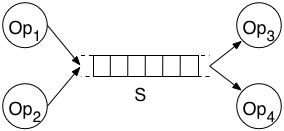
\includegraphics[width=0.45\textwidth]{logical-stream}
    \caption[CoDeR Data Stream]{A stream of the CoDeR data model, contributed to by two sources and consumed from by two sinks.}
    \labelfig{CoDeR: stream}
  \end{figure}

  As has been noted in \refdef{CoDeR: graph instance}, the interval ${[e,n)}$ for any graph instance is the the period of time for which that graph instance is \emph{valid} \citep{SemanticStreamingManagement,sparkwave}.
  The notion of validity within WC-RIF-Core programs relates to the period of time for which a given fact instance ${\langle f, t \rangle}$ is justified by a state ${\Pi^{C,r}_i = \langle R, F^0 \cup B^0 \cup \mathop{\cup}^s_{x=1} W^{S_x,r_x}_i \rangle \models \langle f, t \rangle}$ of a program $\Pi^{C,r}$.
  As such, the interval ${[e,n)}$ is used to express the window ranges $r_x$ for $x \in [1,s]$ of the ${\Pi^{C,r} = \langle R, F^0 \cup B^0, \{ W^{S_x,r_x} \mid x \in [1,s] \} \rangle}$:
  for graph instances entering a CoDeR-based system, $e$ is the instant at which every fact in the given graph was asserted, and $n$ is the instant at which they will leave the semantic window over $S_x$ described by $\Pi^{C,r}$ (a.k.a. being ``negated''), where ${n = e + r_x}$ in the general case;
  for graph instances produced by a CoDeR-based system, $e$ is the latest instant at which any fact within the given graph was asserted, and $n$ is the earliest instant at which any fact within the graph will be negated.
  \reffig{CoDeR: intersected-intervals,CoDeR: consecutive states} provide an example of this for the ${\Pi^{C,3} = \langle \{c \Leftarrow a \land b\},\{\},\{ W^{S,3} \}, 3\rangle}$, where ${S = \langle a,1 \rangle,\langle b,2 \rangle}$ over instants ${i = 1 \dots 4}$.
  \begin{figure}
    \centering
    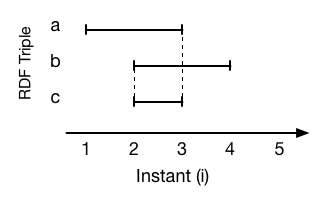
\includegraphics[width=0.4\textwidth]{intersected-intervals-example}
    \caption[Derivation of valid-time for entailed fact instance from those of its justification]{Derivation of valid-time for entailed fact instance \emph{c} from those of its justification \emph{a} and \emph{b}.}
    \labelfig{CoDeR: intersected-intervals}
  \end{figure}
  \begin{figure}[h!]
    \centering
    \begin{align*}
      \Pi^{C,3}_{1} & = \langle \{c \Leftarrow a \land b\}, \{ \langle a, 1 \rangle \} \rangle & \models & \{ \} \\
      \Pi^{C,3}_{2} & = \langle \{c \Leftarrow a \land b\}, \{ \langle a, 1 \rangle, \langle b, 2 \rangle \} \rangle & \models & \{ \langle c, 2 \rangle \} \\
      \Pi^{C,3}_{3} & = \langle \{c \Leftarrow a \land b\}, \{ \langle a, 1 \rangle, \langle b, 2 \rangle \} \rangle & \models & \{ \langle c, 2 \rangle \} \\
      \Pi^{C,3}_{4} & = \langle \{c \Leftarrow a \land b\}, \{ \langle b, 2 \rangle \} & \models & \{ \}
    \end{align*}
    \caption{Consecutive states of a WC-RIF-Core program and their entailments}
    \labelfig{CoDeR: consecutive states}
  \end{figure}

  The first class of CoDeR streams, input/output streams, provide the semantics of the streams and sets $S_x$, $P$, $N$, $F^0$ and $E^0$, for any ${\Pi^{C,r} = \langle R,F^0,\{W^{S_x,r_x} \mid x \in [1,s]\} \rangle \models \langle E^0, P, N \rangle}$ expressed by a CoDeR-based system.
  These streams and sets are represented as CoDeR streams, as per \refdef{CoDeR: stream}, that are, in the case of input streams, produced elsewhere in the Semantic Web or, in the case of output streams, exposed on the Semantic Web as a resource themselves, as per \refdef{CoDeR: input/output}.
  \begin{definition}[Input/Output Stream]\labeldef{CoDeR: input/output}
    Both \emph{input} and \emph{output} streams of CoDeR are CoDeR streams that are identified on the Semantic Web by IRIs.
    The graphs of which there are instances in an input/output stream are heterogeneous, in so much as each graph may contain any number of triples, each in turn being composed of any values.
  \end{definition}
  In each CoDeR-based system the input streams express the logical streams $S_x$ for $x \in [1,s]$ of the given $\Pi^{C,r}$, and a single output stream expresses the logical stream $P$ entailed by the $\Pi^{C,r}$.
  This single output stream also expresses the stream $N$ entailed by the $\Pi^{C,r}$, as that logical stream is defined as the set of instances in the stream $P$ ordered in a sequence by the instant $n$ at which ${\langle R, F^0 \cup B^0 \cup \mathop{\cup}^s_{x=1} W^{S_x,r_x}_{n}}$ \emph{ceased} to justify them;
  this instant $n$ is, therefore, the same $n$ with which each graph is annotated in CoDeR, being the instant at which the graph instance will cease to be valid.
  As such, the annotation of streamed RDF graphs with the interval ${[e,n)}$ gives \emph{all} streams of CoDeR a dual semantics with regard to WC-RIF-Core.

  In addition, the fact instances of $F^0$ are expressed as another input stream $S_0$ over which there is an infinite-range sliding window, where each graph instance is annotated with the instants ${e = 0}, {n = \infty}$ to indicate that it is valid indefinitely;
  likewise, the fact instances $E^0$ appear at the start of the output stream, naturally annotated with the instants ${e = 0}, {n = \infty}$.

  Where many stream processing tasks (including continuous querying) are one-pass, the process of reasoning and inference is iterative/recursive.
  This theoretically necessitates the union of the output stream with the input stream ``upstream'' of the remaining operators of any processing plan in the form of a \emph{working stream}, as per \refdef{CoDeR: working stream}.
  \begin{definition}[Working Stream]\labeldef{CoDeR: working stream}
    The \emph{working stream} of a CoDeR-based system is a CoDeR stream that is the union of all the system's input streams and its output stream.
    It facilitates the \emph{iterative} application of the rules of the system to the streamed data, in the same manner as the \emph{working memory} of the Rete algorithm \citep{forgy79}.
  \end{definition}

  The second class of streams, inter-operator streams, are CoDeR streams that are both produced and consumed exclusively by the stream-to-stream operators of CoDeR's minimal algebra.
  These streams are sequences of the intermediate results of processing between steps in the production of entailments.
  As the production of entailments in CoDeR is cast as an iterative pattern matching problem, all intermediate results of this process will also take the form of instances of RDF graphs.
  However, unlike the graph instances in input and output streams, all instances in a given inter-operator stream will be of graphs that match the same sequenced graph pattern, as per \refdef{CoDeR: sequenced pattern}, yielding \refdef{CoDeR: inter-operator} for inter-operator streams.
  \begin{definition}[Sequential Conjunction]\labeldef{CoDeR: sequential conjunction}
    \emph{Sequential conjunction} is the restriction of conventional conjunction to express not only that two facts are true, but that one precedes the other, for some notion of weak precedence.
    In the context of CoDeR, where the validity of facts changes over time, the sequential conjunction of one fact $a$ with another $b$ is definable as in \refeqn{CoDeR: seq}.
    \begin{equation}
      \labeleqn{CoDeR: seq}
      a\ seq\ b \equiv
        \begin{split}
          a \in g_a & \land \\
          b \in g_b & \land \\
          \langle g_a, e_a, n_a \rangle & \land \\
          \langle g_b, e_b, n_b \rangle & \land \\
          e_a \leqslant e_b < min\left( n_a , n_b \right) &
        \end{split}
    \end{equation}
    This means that not only are $a$ and $b$ valid at the same instant, but $a$ became valid during an instant prior to (or the same as) that at which $b$ became valid.
    For example, if we replace the rule ${c \Leftarrow a \land b}$ in the continuous program \reffig{CoDeR: consecutive states} with ${c \Leftarrow a\ seq\ b}$, then the entailment of each state (and so the streamed entailment of the program) would remain unchanged.
    However, if the rule that uses the complementary sequential conjunction ${c \Leftarrow b\ seq\ a}$ were substituted into that program, then its entailment would be empty, because $a$ strictly preceded $b$.
  \end{definition}
  \begin{definition}[Sequenced Pattern]\labeldef{CoDeR: sequenced pattern}
    A \emph{sequenced pattern} is a SPARQL advanced graph pattern \citep{w3csparql}, extended with the notion of ordering between the components of the graph pattern.
    Where SPARQL graph patterns may be composed using explicit disjunction (UNION and OPTIONAL clauses) or implicit conventional conjunction, sequenced graphs may also make use of explicit \emph{sequential conjunction} between its constituent components, as per \refdef{CoDeR: sequential conjunction}, where each component may be a triple pattern or another sequenced graph pattern.
    As such, the set of all sequenced graph patterns completely subsumes the set of advanced graph patterns of SPARQL, those being sequenced graph patterns that make no use of sequential conjunction.
    
    Sequential conjunction in graph patterns is expressed as a binary clause, SEQ, similar to ${seq}$ in EP-SPARQL \citep{EP-SPARQL}:
    given a sequenced pattern ${\{x\ SEQ\ y\}}$ composed of the sequential conjunction of two subgraph patterns $x$ and $y$, any graph that matches the pattern must contain one subgraph $a$ that matches the pattern $x$ and another subgraph $b$ that matches the pattern $y$, where $a$ must have become valid before (or simultaneously with) $b$.
  \end{definition}
  \begin{definition}[Inter-Operator Stream]\labeldef{CoDeR: inter-operator}
    The \emph{inter-operator} streams of CoDeR are CoDeR streams that are each associated with a specific \emph{sequenced graph pattern} that is a sub-pattern of the body of one of the rules $R$.
    The graphs of which there are instances in an inter-operator stream are homogeneous with respect to the graph pattern associated with that stream, in so much as every such graph is a ``match'' for that graph pattern, as per \refdef{CoDeR: sequenced pattern}.
    While the ordering in a sequenced graph pattern is not represented directly in the graph instances matched, those being temporally-annotated RDF graphs, the nature of the processing that produces a given graph instance may dictate a \emph{necessary ordering} between the components of every graph instance that it produces (see \refsec{CoDeR: SteM}).
    It is this \emph{necessary ordering} that is represented by the ordering in a sequenced graph pattern.
  \end{definition}
  It should be noted that, by \refdef{CoDeR: sequenced pattern} of sequenced patterns, the conventional conjunction between two patterns $a$ and $b$ is semantically equivalent to the disjunction of two graph patterns that are complementary sequential conjunctions between the two component patterns, as shown in \refeqn{CoDeR: disjunction of sequential conjunctions}.
  As such, any SPARQL graph pattern may be expressed without the use of conventional conjunction.
  \begin{equation}
    \labeleqn{CoDeR: disjunction of sequential conjunctions}
    \{a\ SEQ\ b\}\ UNION\ \{b\ SEQ\ a\} \equiv \{a\ .\ b\ .\}
  \end{equation}
  
  It follows that the distinction between input/output streams and inter-operator streams is one of semantics, rather than functionality.
  Both are, syntactically, CoDeR streams as per \refdef{CoDeR: stream}.
  Semantically, the contents of input streams are the assertions of the predecessor of a CoDeR-based system in a wider stream processing pipeline, as identified on the Semantic Web by an IRI, and cannot be expected to match any given pattern.
  It follows that the same is true of the output stream, as the entire contents of all input streams is part of the entailment of a WC-RIF-Core program.
  In contrast, the contents of inter-operator streams are not expected, in the general case, to hold any intrinsic value outside of a system (though there is no reason it should not be exposed on the Semantic Web);
  instead, they contain the intermediate result of some highly specific part of the inference over the program expressed by the system, represented by a sequenced graph pattern.
  \end{nestedsection}

  % Minimal Algebra
  \begin{nestedsection}{An Algebra for CoDeR}{model: algebra}
    An algebra for CoDeR is any set of operators fit for the purpose of describing the process of continuous inference, as expressed in any WC-RIF-Core program, over CoDeR streams.
    In this section we present such a set of operators, detailed individually with regards to the nature of the CoDeR streams that each produces and may be applied to, as well as the specific actions that each takes with respect to each graph instance it receives.
    We go on to present the transformations of expressions in this algebra that support the optimisation of processing WC-RIF-Core programs.

    The algebra fundamentally consists of the following set of stream-to-stream operators: ${\{{}_g\pi_t, \sigma_{triple}, \sigma_{external}, \coloneq_{head}, \cup, \rstreamjoin\}}$.
    These operators encapsulate the practical expression of the set of functions required to derive the entailment of WC-RIF-Core programs in the context of CoDeR input/output streams.
    These functions are those required for WC-Datalog programs, with the addition of two functions:
    a one-pass unary evaluation function $\sigma_{external}$ for the built-in predicates of RIF-Core;
    and a one-pass unary graph decomposition function ${{}_g\pi_t}$ to convert the CoDeR input stream of heterogeneous RDF graph instances into a stream of homogeneous RDF triple instances, the latter being the form of a stream $S_x$ of a program ${\Pi^{C,r} = \langle R, F^0, \{ W^{S_x, r_x} \mid x \in [1,s] \} \rangle}$.
    The continuous derivation of the entailment of WC-Datalog programs requires, in turn, the set of functions required for querying deductive databases using Datalog, with the addition of another two functions:
    a two-pass unary valid-window maintenance function $w$ to enforce the windows of range $r_x$, for $x \in [1,s]$, over the CoDeR input streams;
    and a two-pass unary window-to-stream function $s$ to extract the stream of novel graph instances from a sequence of consecutive valid-windows, closely related to the ${IStream()}$ function of CQL \citep{StanfordStream}.
    Finally, the functions required for querying deductive databases using Datalog are conventionally the complete set required of the relational algebra\footnote{This refers to the complete relational algebra less the functionality of set minus $\setminus$, which is analogous to the NaF operator $\sim$ that is not supported by positive Datalog.}, being ${\{\sigma,\pi,\Join,\cup\}}$ as described by \citet{codd70relationalModel}.
    However, three of these may be restricted when processing semantic data, becoming:
    the one-pass unary equality-based triple-select $\sigma_{triple}$;
    the two-pass binary natural join $\Join^\ast$ between \emph{sets} of variable bindings for graph patterns (requiring valid-windows over streams as input, and producing valid-windows);
    and the one-pass unary template-project $\pi_{triple}$ that projects constant values and bindings for variables in graph patterns from graph instances into new triple instances.
    The one-pass binary set operator $\cup$ utilised by the relational algebra need only be modified to preserve the mapping of instances to instants when applied to CoDeR streams.

    All one-pass functions required to derive the entailment of a WC-RIF-Core program expressed by an equivalent stream-to-stream operator in CoDeR, as detailed in \reftab{WC-RIF-Core-functions-to-CoDeR-operators}.
    \begin{table*}
        \centering
        \begin{tabular}{r || c | c | c | c | c | c | c | c}
          WC-RIF-Core & $\sigma_{triple}$ & $\sigma_{external}$ & ${}_g\pi_t$ & $\pi_{triple}$ & $\cup$ & $w$ & $s$ & $\Join^\ast$ \\ \hline
          CoDeR & $\sigma_{triple}$ & $\sigma_{external}$ & ${}_g\pi_t$ & $\coloneq_{head}$ & $\cup$ & \multicolumn{3}{c}{$\rstreamjoin \cup \rstreamjoin$}
        \end{tabular}
        \caption[WC-RIF-Core Functions to CoDeR Operators]{The mapping of each function of WC-RIF-Core to their expression using the operators of the CoDeR algebra.}
        \labeltab{WC-RIF-Core-functions-to-CoDeR-operators}
      \end{table*}
      The two-pass functions $\{w,s,\Join^\ast\}$, as shown in the same table, are combined into a single stream-to-stream operator in CoDeR in order to make the algebra universally stream-to-stream in nature.
      This is possible because $w$ is solely used to produce a set from a stream, $s$ to produce a stream from a set, and $\Join^\ast$ is the only function that must specifically act between sets;
      it follows that the former two will always, and need only, be used in direct conjunction with the latter in the form $s(w(X) \Join^\ast w(Y))$, where $X$ and $Y$ are inter-operator streams.

    As all the operators of this algebra are stream-to-stream in nature, they each receive one or two streams and produce a single stream.
    As such, the notation for applying an operator to a stream is also the definition of a stream, and may, therefore, be the argument for another operator.
    % , termed the \emph{successor} operator, as per \refdef{CoDeR: successor operator}.
    % For example, \refeqn{basic-example-plan} is a plan for the ${\Pi^{C,r} = \langle \{b \Leftarrow a\}, \{\}, S, r \rangle}$ expressed in the CoDeR algebra, where $a$ and $b$ are RDF triples.
    % \begin{equation}\labeleqn{basic-example-plan}
    %   \coloneq_b \left( \sigma_a \left( {}_g{\pi_t}\ S \right) \right)
    % \end{equation}
    % In this case, $\sigma_a$ is the successor operator of ${{}_g\pi_t}$, and is succeeded by $\coloneq_b$ in turn.

    % \begin{definition}[Successor Operator]\labeldef{CoDeR: successor operator}
    %   A \emph{successor} of an operator $a$ is any operator $b$ that receives the stream produced by $a$, i.e. $b \left( a \left( S \right) \right)$ for some suitable stream $S$.
    %   This relationship is denoted ${a \circ b}$, as it is analogous to operator composition, and may be chained to represent extended operator pipelines, e.g. ${a \circ b \circ c}$.
    %   Where an asymmetric binary operator is a successor, the succeeding function of the operator is noted above the successor symbol, e.g. ${{}_g\pi_t \circ \sigma_p \overset{build}{\circ} \rstreamjoin}$, where $p$ is some triple pattern.
    % \end{definition}

    The following descriptions present a thorough treatment of the individual operators of the algebra.
    Each provides a description of its behaviour on a triple-by-triple basis, and the formal definition of the stream produced in terms of the stream(s) to which the operator is applied.
    Many of the operators' behaviours are defined in terms of bindings within graph instances for variables in the sequenced pattern associated with a received stream;
    to represent this relationship between streams/patterns and the graphs/propositions that match them we use the same notation of an \emph{extended variable substitution} $\bar{s}$ used in the satisfaction of $\ast$-Datalog programs.

    \begin{nestedsection}{Graph-to-Triples}{CoDeR: graph-to-triples}
      \begin{figure}
        \centering
        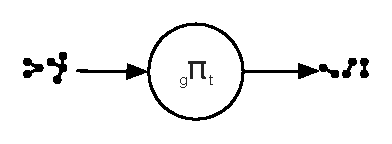
\includegraphics[width=0.3\textwidth]{graph-to-triple}
        \caption{The graph-to-triple operator.}
        \labelfig{CoDeR: graph-to-triple}
      \end{figure}
      The graph-to-triples operator ${{}_g\pi_t}$ is a one-pass unary operator that deconstructs graph instances into sequences of triple instances, the union of those triples instantiated being equal to the contents of the original graph.
      It takes an \emph{input} stream $X$ and produces an \emph{inter-operator} stream ${{}_g\pi_t\ X}$, whose associated pattern is always the singleton pattern ${\{?subj\ ?pred\ ?obj\ .\}}$.

      Each singleton graph instance on the produced stream is composed of a triple drawn from a received graph instance and the same valid-time interval as that graph instance.
      Consider, for example, the input stream containing an instance of a graph containing the RDF triples $a$ and $b$ and valid from instant $e$ to instant $n$:
      \begin{multline*}
        {}_g{\pi_t} (\dots,\langle \{a\ .\ b\ .\},e,n \rangle,\dots) = \\
          (\dots,\langle \{a\ .\},e,n \rangle,\langle \{b\ .\},e,n \rangle,\dots)
      \end{multline*}
      More generally:
      \begin{equation*}
        {}_g{\pi_t} \left( X \right) =
        \left(
          \langle \{t .\}, e, n \rangle \:\middle\vert\: \langle g, e, n \rangle \in X \land t \in g
        \right)
      \end{equation*}
    \end{nestedsection}
    \begin{nestedsection}{Triple-Select}{CoDeR: triple-select}
      The triple-select operator identifies instances of triples in a stream $X$ that match some \emph{triple pattern} \citep{w3csparql}.
      This operator is semantically equivalent to the \emph{basic pattern match} of SPARQL applied to a stream of triple instances, rather than a set of triples, and to the \emph{alpha nodes} of the Rete pattern matching algorithm \citep{forgy79} applied to temporally annotated semantic data.
      Like these operators, the triple-select is one-pass, and so is trivially interpreted as the unary stream-to-stream operator $\sigma_{triple}$, where ${triple}$ is the triple pattern to be matched.
      \begin{figure}
        \centering
        
\includegraphics[width=0.3\textwidth]{basic-pattern-match}
        \caption{The triple-select operator.}
        \labelfig{CoDeR: basic pattern match}
      \end{figure}

      The triple-select takes an inter-operator stream $X$ of singleton graph instances and produces an inter-operator stream, where the produced stream contains a subset of those instances in the received stream and maintains the ordering of those instances.
      The set of instances produced is defined as the subset of those received that contains only those singleton graph instances for whom the single triple matches the specified triple pattern.

      More formally, where ${matches(graph,pattern)}$ is true iff the $graph$ matches the $pattern$ as per \refdef{CoDeR: sequenced pattern}:
      \begin{equation*}
        \sigma_{triple} \left( X \right) =
        \left(
          \langle g, e, n \rangle
        \:\middle\vert\:
          \begin{split}
            \langle g, e, n \rangle \in X & \land \\
            \exists \bar{s} \left(
              \bar{s}\left( \{ triple\ .\} \right) = g
            \right)
          \end{split}
        \right)
      \end{equation*}
    \end{nestedsection}
    \begin{nestedsection}{External-Select}{CoDeR: external-select}
      The external-select operator encompasses all of the one-pass built-in datatype predicates and functions of RIF-Core.
      Like the triple-select, it is trivially interpreted as a unary stream-to-stream operator $\sigma_{external}$, where ${external = f(a_1,\dots,a_n)}$, $f$ is one of the built-in predicates of RIF-Core and each $a_i$, ${1 \leq i \leq n}$, is either a variable, a constant value or a built-in function of RIF-Core to which $f$ is to be applied.
      \begin{figure}
        \centering
        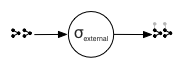
\includegraphics[width=0.3\textwidth]{datatype-function}
        \caption{The operator encompassing all datatype functions of RIF-Core.}
        \labelfig{CoDeR: datatype function}
      \end{figure}
      It should be noted that the built-in functions of RIF-Core resemble the built-in predicates, but evaluate to a value rather than either ${true}$ or ${false}$, and so are only valid as arguments to another built-in predicate or function.
      The $\sigma_{external}$ filters elements of its received stream $X$ based not on the semantic structure of the data but directly on the values bound within each graph instance for variables of the graph pattern of $X$;
      thus the $\sigma_{external}$ operator not only expresses the built-in predicates and functions of RIF-Core but is analogous to the non-NaF FILTER clauses of \emph{advanced graph patterns}, as specified in SPARQL.

      The external-select takes an inter-operator stream $X$ and produces an inter-operator stream of graph instances, where the produced stream contains a subset of those instances in the received stream and maintains the ordering of those instances.
      The contents of the produced stream are characterised as those graph instances from the received stream whose graphs match the sequenced pattern that is the conventional conjunction of the pattern of $X$ and the proposition ${external}$.
      The sequenced pattern associated with stream $X$ must contain all the variables referenced as arguments that must be bound in the proposition ${external}$ \citep{w3crifcoreBuiltins}, as the proposition will always evaluate to false where not all necessary arguments are bound.
      As such, the produced stream will necessarily be the empty stream $\varnothing$, as per \refdef{CoDeR: empty stream}.

      More formally:
      \begin{equation*}
        \sigma_{p} \left( X \right) =
        \left(
          \langle g, e, n \rangle
        \:\middle\vert\:
          \begin{split}
            \langle g, e, n \rangle \in X & \land \\
            \exists \bar{s} \left(
              \begin{split}
                \bar{s}\left( X \right) = g & \land \\
                \bar{s}\left( p \right) &
              \end{split}
            \right)
          \end{split}
        \right)
      \end{equation*}
    \end{nestedsection}
    \begin{nestedsection}{Instance Implication}{CoDeR: instance implication}
      \begin{figure}
        \centering
        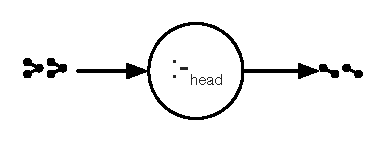
\includegraphics[width=0.3\textwidth]{instance-implication}
        \caption{The instance implication operator.}
        \labelfig{CoDeR: instance implication}
      \end{figure}
      Instance implication $\coloneq_{head}$ is a one-pass unary operator that takes an inter-operator stream $X$ whose associated pattern is the body of one of the rules $R$ of the expressed $\Pi^{C,r}$, and produces an inter-operator stream whose associated pattern is the head of that axiomatic rule, ${head}$.
      Each graph instance received on $X$ causes the production of a single graph instance that matches the pattern of the head clause and is populated with the values bound to the pertinent variables within the received instance.
      This is similar to the CONSTRUCT clause of SPARQL, or the final step of \emph{conflict set resolution} within the Rete algorithm \citep{forgy79}.
      In addition, each produced instance inherits its valid-time interval from the graph instance from which it is derived.

      More formally, using the example case of a singleton graph pattern ${head = \{ a_0\ a_1\ a_2\ .\}}$ for readability:
      \begin{equation*}
        \coloneq_{head} \left( X \right) =
        \left(
          \langle h, e, n \rangle
        \:\middle\vert\:
          \begin{split}
            \langle g, e, n \rangle \in X & \land \\
            \exists \bar{s} \left(
              \begin{split}
                \bar{s}\left( X \right) = g & \land \\
                \bar{s}\left( head \right) = h &
              \end{split}
            \right)
          \end{split}
        \right)
      \end{equation*}
    \end{nestedsection}
    \begin{nestedsection}{Stream Union}{CoDeR: stream union}
      Stream union is a one-pass binary operator $\cup$, meaning that it takes two streams and produces a single stream that is composed of all the mappings of instances to times from both received streams.
      No new instances are created by the stream union operator, unlike the projection-like operators ${{}_g\pi_t}$ and $\coloneq_{head}$, nor are any instances filtered from the received stream, unlike the select-based operators $\sigma_{triple}$ and $\sigma_{external}$.
      Both the streams received and the stream produced may be either input/output streams or inter-operator streams, but the produced stream may only be an inter-operator stream if \emph{both} of its received streams are as well:
      if one of the received streams is not an inter-operator stream then there is no way to reliably define the pattern matched by each instance in the produced stream, as is necessary for an inter-operator stream.

      More formally:
      \begin{equation*}
        \left( X \right) \cup \left( Y \right) =
        \left(
          \langle g, e, n \rangle
        \:\middle\vert\:
            \begin{split}
              \langle g, e, n \rangle \in X & \lor \\
              \langle g, e, n \rangle \in Y
            \end{split}
        \right)
      \end{equation*}

      As shown in \reffig{CoDeR: stream union}, this algebraic operator does not have an operator node to represent it in dataflow representations of a processing plan.
      \begin{figure}
        \centering
        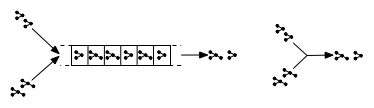
\includegraphics[width=0.45\textwidth]{stream-union}
        \caption{The expression of stream union in CoDeR as the contribution of multiple operators to the same stream.}
        \labelfig{CoDeR: stream union}
      \end{figure}
      This is because the multi-source and in-order natures of CoDeR data streams allows for the behaviour of $\cup$ to be expressed passively through those streams, rather than within a distinct data processing operator.
    \end{nestedsection}
    \begin{nestedsection}{SteM}{CoDeR: SteM}
      State Modules were originally proposed in the adaptive continuous processing literature, and their potential implementations for static and sliding-window datasets are thoroughly detailed by \citet{SteMs}.
      In CoDeR they are asymmetrical binary operators, represented algebraically by the binary operator $\rstreamjoin$, that simply supports the maintenance (or ``building'') of a \emph{valid window}, as per \refdef{continuous datalog: valid window}, from one inter-operator stream and naturally joining each graph instance on a second inter-operator stream against those within the maintained window (known as ``probing'' the window).
      Since the persistent fact instances of $F^0$ are simply included as the CoDeR input stream $S_0$ and are annotated as being perpetually valid, as discussed in \refsec{model: data}, the applicable part of $F^0$ (and its entailment with respect to the rules $R$) will be perpetuated indefinitely in each SteM.
      The nature of probing in CoDeR is the same as that of joining the sets of matches for two graph patterns in SPARQL.
      As such, ${X \rstreamjoin Y}$ produces an inter-operator stream of graph instances rather than a stream of tuple instances that would be produced by a conventional natural window-join.

      Building and probing a window are the same two functions performed for each window in a symmetric natural window-join (that shall be noted as the operator ${X \Join^\ast_w Y}$ in this section), as discussed by \citet{niagaraCQ} and extended from Rete \emph{beta nodes} in \citep{ReteDBMS}, with results of probing each window being produced to the same result stream.
      \begin{figure}
        \centering
        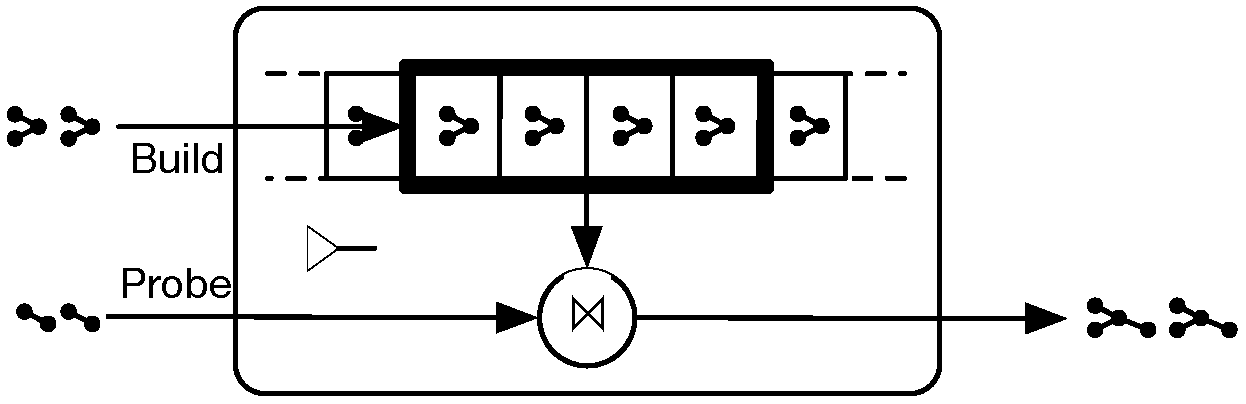
\includegraphics[width=0.45\textwidth]{SteM}\\
        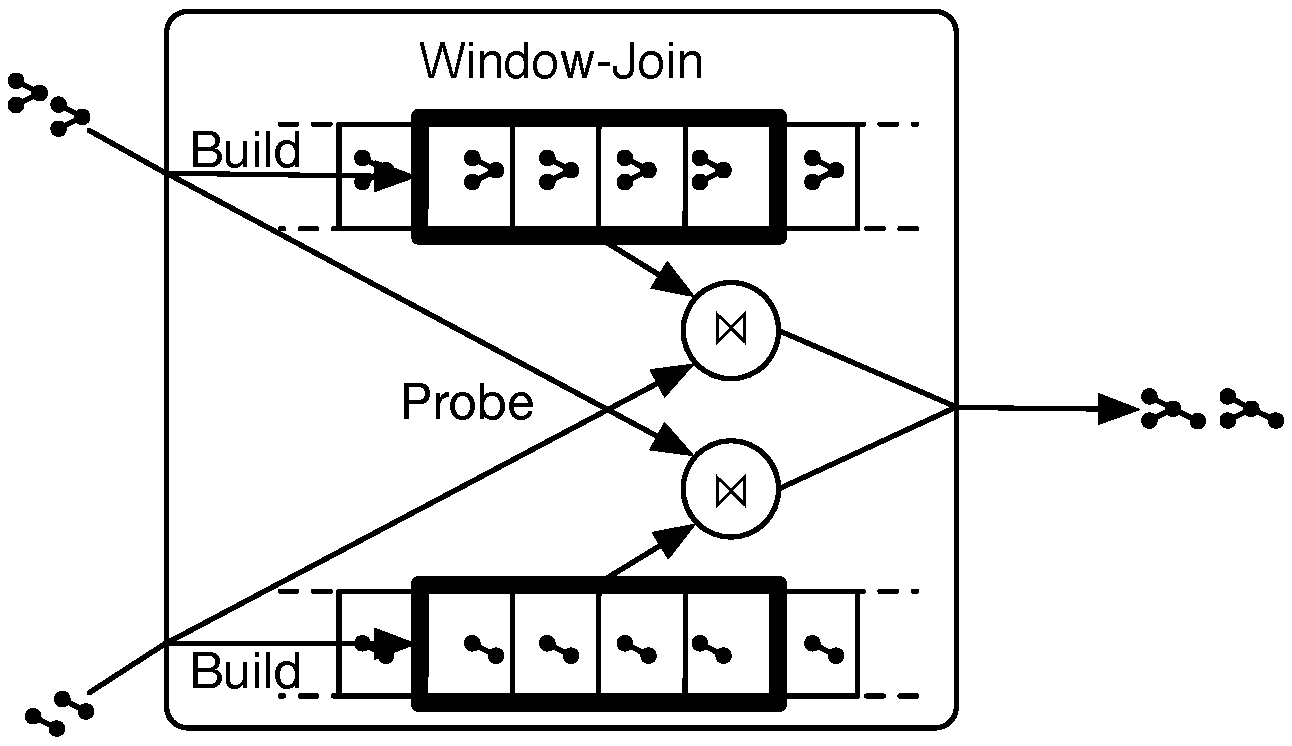
\includegraphics[width=0.45\textwidth]{window-join}
        \caption{Exploded views of two-pass joining stream operators.}
        \labelfig{CoDeR: SteM}
      \end{figure}
      Therefore, natural window-joins are functionally identical to the stream union of two \emph{complementary} SteMs (i.e. ${X \rstreamjoin Y}$ and ${Y \rstreamjoin X}$) applied to inter-operator streams, as in \refeqn{window-join-from-union-of-SteMs}.
      \begin{equation}\labeleqn{window-join-from-union-of-SteMs}
        X \Join^\ast_w Y = \left( X \rstreamjoin Y \right) \cup \left( Y \rstreamjoin X \right)
      \end{equation}
      In addition, it should be noted that SteMs express the semantics of the sequential join operator ${seq}$ proposed in EP-SPARQL \citep{EP-SPARQL}, in that they join new data from one stream with the prior (valid) contents of another, thereby supporting rudimentary event processing.
      As such, the sequenced pattern associated with the stream produced by ${X \rstreamjoin Y}$ would be ${\{x\ SEQ\ y\}}$, as per \refdef{CoDeR: sequenced pattern}, where $x$ is the pattern associated with stream $X$, and $y$ is the pattern associated with $Y$.
      This leads to the isomorphism between \refeqn{CoDeR: disjunction of sequential conjunctions,window-join-from-union-of-SteMs}.

      Finally, in contrast to the direct inheritance of valid-times in ${{}_g\pi_t}$ and $\coloneq_{head}$, the valid-time interval assigned to each graph produced by a SteM is the intersection of the valid-times of the two unioned graphs.  More formally:
      \begin{equation*}
        \left( X \right) \rstreamjoin \left( Y \right) =
        \left(
          \langle g, e_Y, n_m \rangle \:\middle\vert\:
          \begin{split}
            \langle g_X, e_{X}, n_{X} \rangle \in X & \land \\
            \langle g_Y, e_{Y}, n_{Y} \rangle \in Y & \land \\
            e_{X} \leqslant e_{Y} < n_{X} & \land \\
            \{g_X\} \Join^\ast \{g_Y\} = \{g\} & \land \\
            n_m = min \left( n_{X}, n_{Y} \right) &
          \end{split}
        \right)
      \end{equation*}
    \end{nestedsection}

  %   \begin{nestedsection}{Transformations}{CoDer: transformations}
  %     As is the case with relations in the relational algebra, the same stream may be defined in a variety of ways using the set of operators.
  %     As each inter-operator stream is associated with a sequenced pattern, each definition of a stream may also be called a \emph{plan} for matching that stream's pattern.
  %     Such equivalences between plans rely on a set of fundamental equivalences known as \emph{transformations}.
  %     The most fundamental of the transformations of the relational algebra are traditionally classified as \emph{identity}, \emph{commutative}, \emph{associative} or \emph{distributive}, all of which apply equally well to the operators of CoDeR due to their similarity to those of SPARQL, which in turn have an equivalence to those of the relational algebra, as discussed by \citet{cyganiak05relationalSPARQL}.

  %     Many of the transformations in this algebra are directly related to those of the relational algebra.
  %     Those applied to selections $\sigma$ and joins $\Join$ are mirrored exactly by those applied to external-selects $\sigma_{external}$ and SteMs $\rstreamjoin$, except for the fact that SteMs are not commutative.
  %     Also, all operators are distributive over stream union, which itself inherits all of the transformations of set union with respect to itself (commutative, associative and identity).
  %     Furthermore, both $\sigma_\ast$ operators of CoDeR are commutative with respect to themselves and each other.
  %     On the other hand, unlike in the relational algebra, triple-selects $\sigma_{triple}$ are not distributive over SteMs, and neither the graph-to-triples ${{}_g\pi_t}$ nor instance implication $\coloneq_{head}$ operators are commutative or distributive over other operators.

  %     In addition, there are a number of identities that allow the elimination of redundant operators from a plan.
  %     These are mostly based on the subsumption of the pattern associated with an inter-operator stream by a $\sigma_\ast$ operator.
  %     For example, if a stream $s$ is produced on which a given variable $?v > x$, then any stream produced by an external-select on the proposition $?v > y \leqslant x$ applied to $s$ will be equal to $s$, making the external-select redundant.
  %     Equally, if a stream $s$ of singleton graphs matches the pattern ${\{ s\ p\ ?o\ .\}}$, then any stream produced by a triple-select $\sigma_{?s\ p\ ?o}$ applied to $s$ will be equal to $s$, making the triple-select redundant.
  %     Finally, a graph-to-triples operator is obviously redundant when applied to an inter-operator stream of singleton-graph instances.
  % \end{nestedsection}
\end{nestedsection}
  
  \begin{nestedsection}{Summary of CoDeR}{CoDeR: summary}
    Given the time-based nature of windowing and of the justification of entailments in WC-RIF-Core, it is possible to determine in advance the instant at which fact instances will be negated.
    Furthermore, facts in RDF may be grouped into graphs, meaning that fact instances with the same annotation that will be negated at the same instant may be grouped into an annotated graph without loss of information.
    As such, both streams $P$ and $N$ entailed by a $\Pi^{C,r}$ may be represented by streams of CoDeR's twice-annotated graphs.
    As the SteM $\rstreamjoin$ is the only CoDeR operator that maintains any form of window over its input, and SteMs maintain exclusively \emph{valid windows}, no data will persist within a CoDeR-based system when it is no longer valid according to its annotations.
    Furthermore, the valid-time interval of any instance is either directly inherited from the interval of the input instance, in the case of one-pass operators, or derived from the intersections of the intervals of both contributing instances in the sole two-pass operator, the SteM;
    as such, it is guaranteed that all instance annotations accurately describe the intervals for which the given instance is justified by the states of a given WC-RIF-Core program ${\Pi^{C,r} = \langle R,F^0 \cup B^0, \{ W^{S_x,r_x} \mid x \in [1,s] \} \rangle}$.

    It follows that no fact instance may persist in a CoDeR based system if it is no longer valid, and thus only entailments that are valid at a given moment may be produced in that moment, thereby guaranteeing correct results according to the semantics of WC-RIF-Core.
    It also follows that, given a system with a processing plan that is expressible in the CoDeR algebra and accurately represents a set of rules $R$ of a $\Pi^{C,r}$, all fact instances that are logically entailed by that $\Pi^{C,r}$ at a given instant will be persisted within that system at that instant,
    i.e. such a CoDeR-based system is guaranteed to produce the complete stream of results according to the semantics of WC-RIF-Core.
  \end{nestedsection}
\end{nestedsection}

\begin{nestedsection}{R4 System: Rule-based Reasoning over RDF streams using Rete}{implementation}
  As a proof of concept for the CoDeR model, we have implemented R4: a Rule-based Reasoner for RDF-streams using Rete.
  Reasoning in R4 is performed continuously and incrementally as dataflow networks that work directly on RDF streams, constructed according to the Rete pattern matching algorithm \citep{forgy79}.
  The system architecture is shown in \reffig{R4-architecture}.
  \begin{figure}[b]
    \centering
    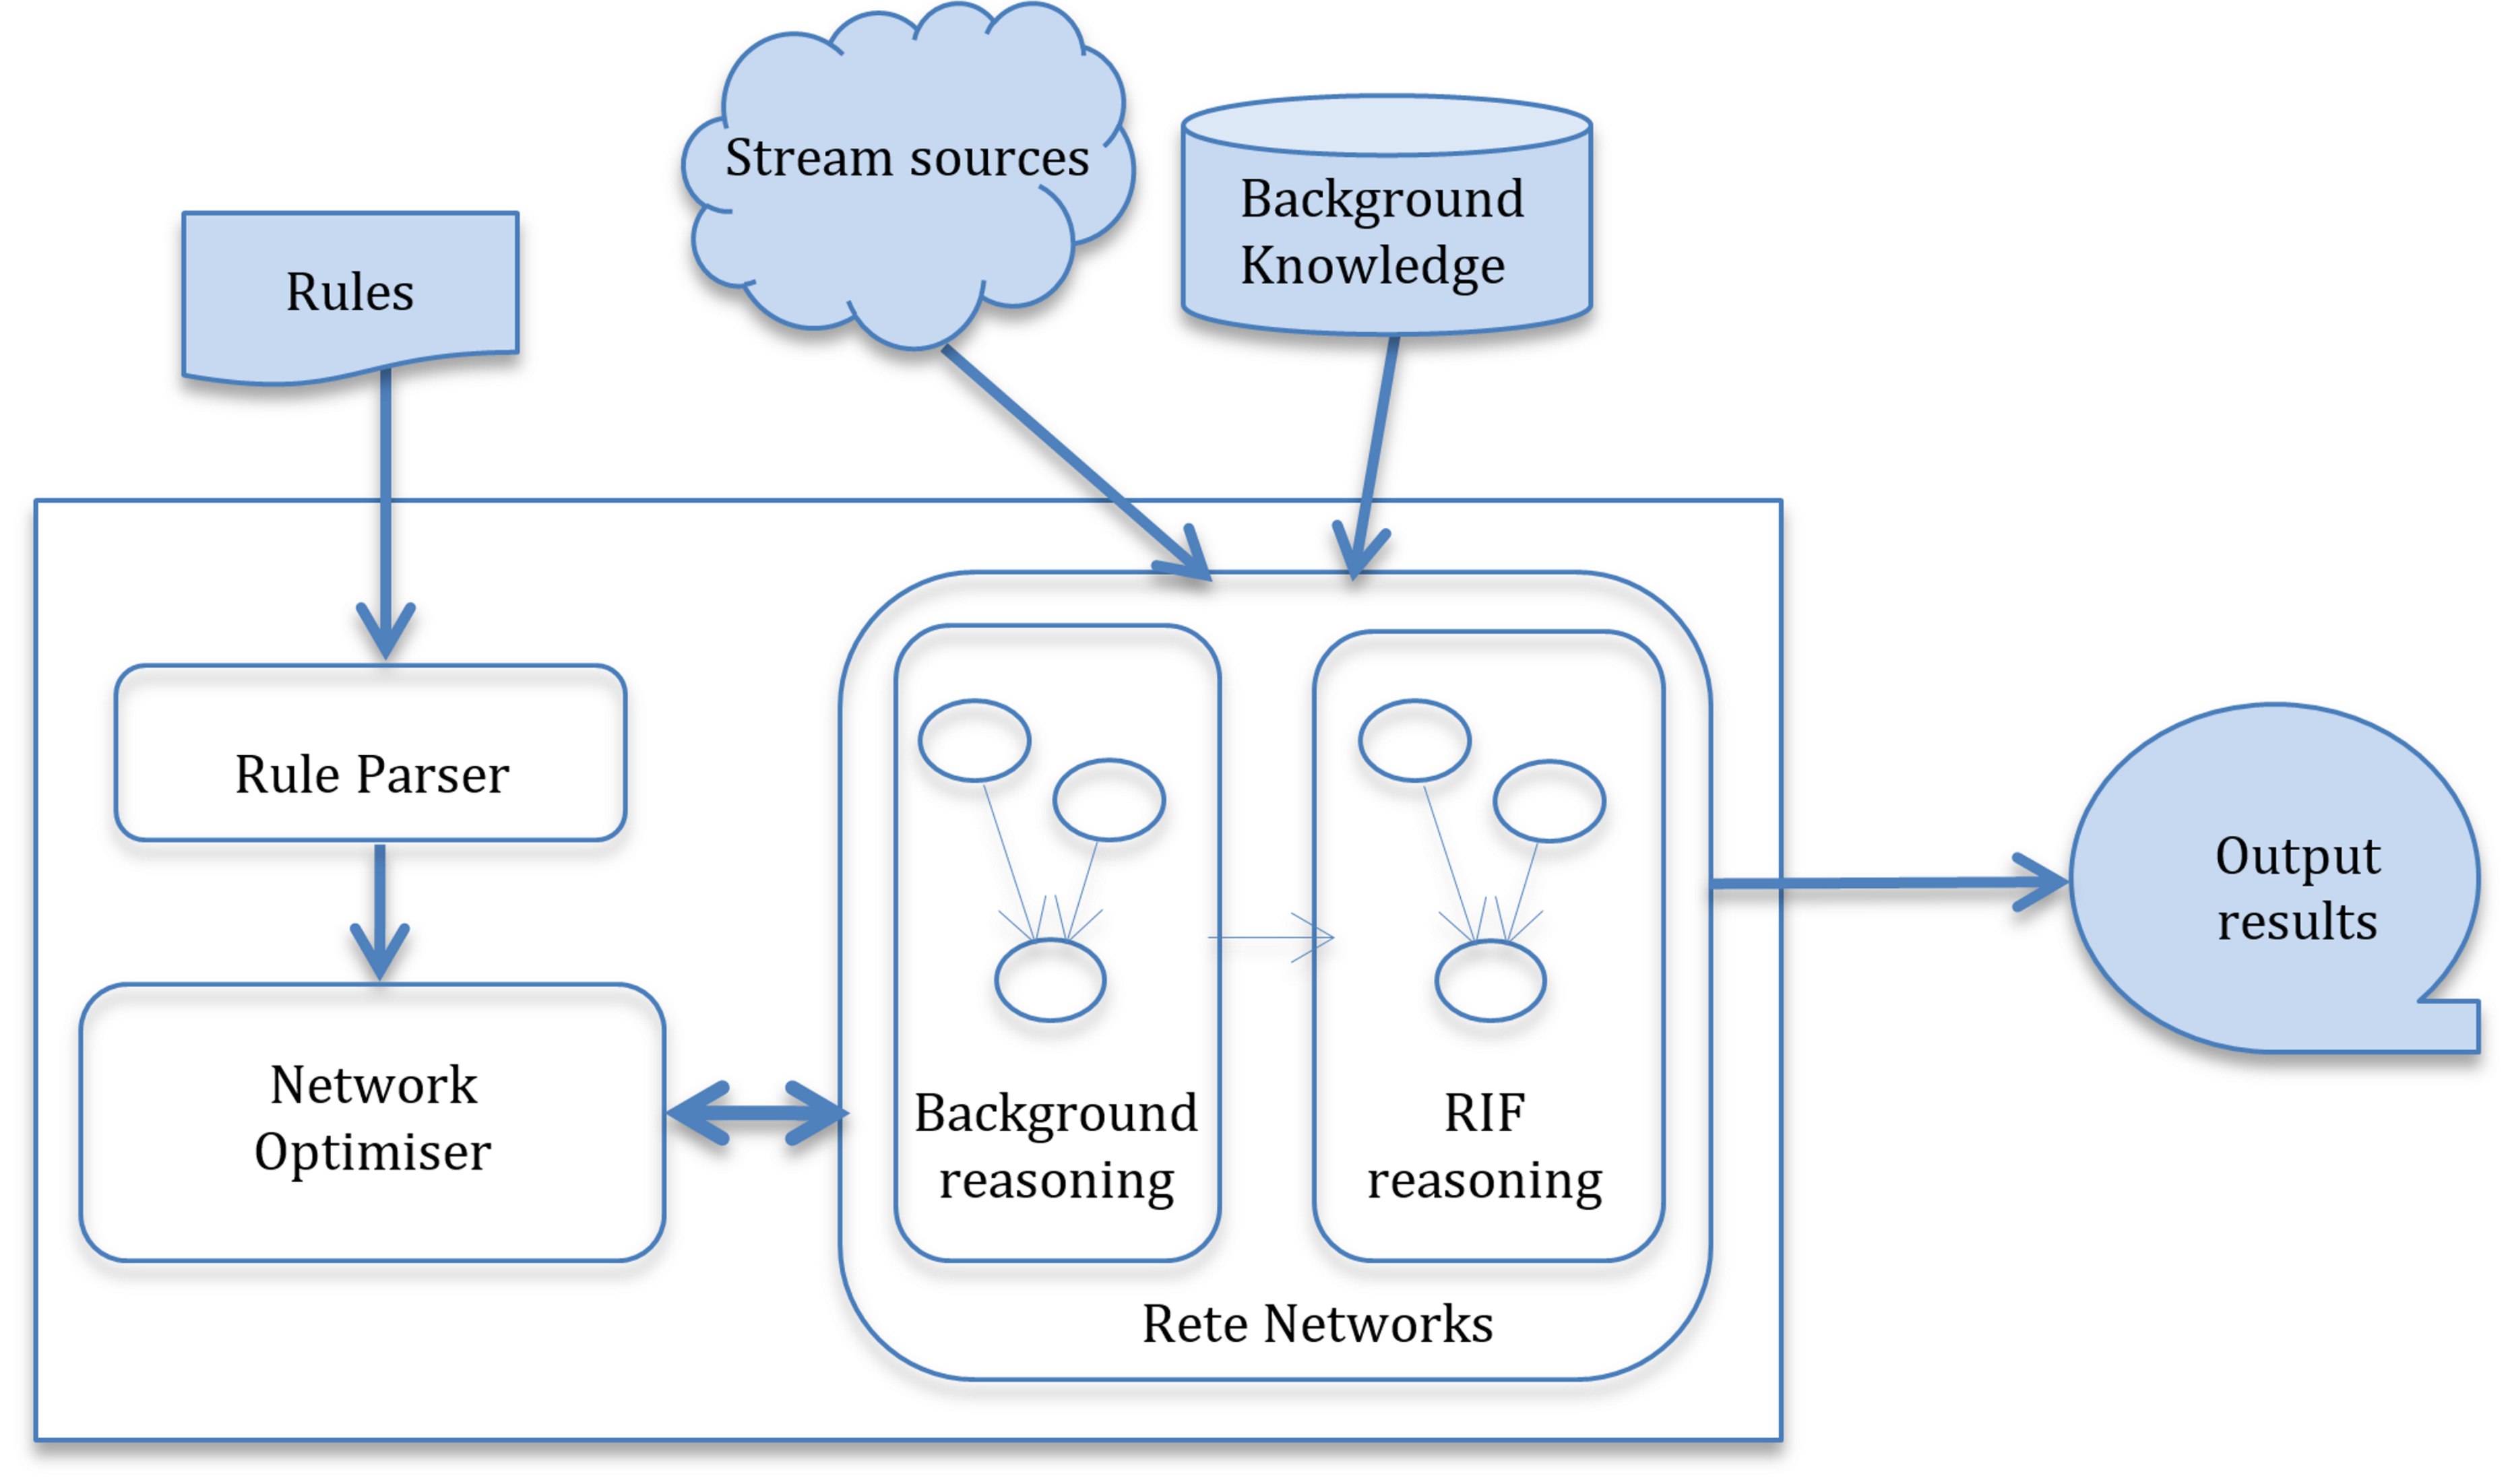
\includegraphics[width=0.45\textwidth]{R4-architecture.png}
    \caption{The system architecture of R4.}
    \labelfig{R4-architecture}
  \end{figure}

  \begin{figure*}[t]
    \centering
    \begin{ebnf}
      \Rule{Document}{
              \Optional{\NTerm{IRIMETA}} 
              \Token{Document} 
              \Token{(} 
              \Optional{\NTerm{Base}} 
              \ZeroOrMore{\NTerm{Prefix}} 
              \ZeroOrMore{\NTerm{Import}}
              \Optional{\NTerm{Window}}
              \Optional{\NTerm{Group}} 
              \Token{)}
      }
      \Rule{Base}{
              \Token{Base} 
              \Token{(} 
              \NTerm{ANGLEBRACKIRI} 
              \Token{)}
      }
      \Rule{Prefix}{
              \Token{Prefix} 
              \Token{(} 
              \NTerm{Name} 
              \NTerm{ANGLEBRACKIRI} \Token{)}
      }
      \Rule{Import}{
              \Optional{\NTerm{IRIMETA}} 
              \Token{Import} 
              \Token{(} 
              \NTerm{LOCATOR} 
              \Optional{\NTerm{PROFILE}} 
              \Token{)}
      }
      \Rule{Group}{
              \Optional{\NTerm{IRIMETA}} 
              \Token{Group} 
              \Token{(} 
              \ZeroOrMore{\OrList{\NTerm{RULE} \OrSep \NTerm{Group}}} 
              \Token{)}
      }
      \Rule{RULE}{
              \Optional{\NTerm{IRIMETA}}
              \Token{Forall}
              \OneOrMore{\NTerm{Variable}}
              \Token{(}
              \NTerm{CLAUSE}
              \Token{)}
      }
      \OrRule{
              \NTerm{CLAUSE}
      }
      \Rule{CLAUSE}{
              \OrList{\NTerm{Implies} \OrSep \NTerm{ATOMIC}}
      }
      \Rule{Implies}{
              \Optional{\NTerm{IRIMETA}}
              \OrList{\NTerm{ATOMIC} \OrSep \Token{And} \Token{(} \ZeroOrMore{ATOMIC} \Token{)}}
              \Token{:-}
              \NTerm{FORMULA}
      }
      \Rule{LOCATOR}{
              \NTerm{ANGLEBRACKURI}
      }
      \Rule{PROFILE}{
              \NTerm{ANGLEBRACKURI} 
      }
      \Rule{Window}{
              \NTerm{Number}
              \NTerm{TimeUnit}
      }
      \Rule{TimeUnit}{
              \OrList{\Token{ms} \OrSep \Token{s} \OrSep \Token{m} \OrSep \Token{h}}
      }
    \end{ebnf}
    \caption{Streaming RIF-Core Grammar}
    \labelfig{lst-S-RIF-Core}
  \end{figure*}

  A rule document containing any number of rules is submitted to the system.
  We have chosen RIF-Core to be the language in which rules can be represented, for being compatible with RDF and other semantic web standards, as well as sharing the semantics of positive Datalog.
  The rule document specifies any domain-specific rules as well as an entailment regime \emph{if any} for background reasoning.
  We also added a simple extension to RIF-Core in line with the extension of Datalog described in \refsec{semantics}, enabling users to specify a window range as part of their rule set, as shown in \reffig{lst-S-RIF-Core}.
  Further, we propose the extension of the set of `PROFILE's that describe the `Import's of a rule set to include those definitions of RDF streams recognised by the W3C.

  These rules are translated by the rule parser into a set of objects that are then used by the network optimizer to generate the Rete-like dataflow networks.
  The optimizer employs simple known heuristics to generate a good plan.
  These heuristics include: sharing nodes between rules where the sub-graph patterns their results match are variants of each other; avoiding Cartesian products as much as possible by joining patterns that have common variables earlier in the beta network; and pushing more selective patterns (those with fewer variables) earlier in the alpha network to minimize intermediate results.
  
  The optimizer instantiates a Rete network for background reasoning if required and another network for generic rules.
  The first network feeds into the second one and the two together are ``re-entrant'', meaning that the first network takes as input the stream of entailments produced by both the first and the second, to enable iterative inference of results such as the calculation of transitive closure.
  
  These networks receive streaming data in the form of sequences of RDF graphs, and operate directly on each of these graphs incrementally.
  We chose this RDF-native approach as opposed to reusing existing technologies as in \citep{C-SPARQL,streaming-sparql} to allow full control over the low-level operators.
  This can offer maximum optimization opportunities such as adaptively optimizing the network topologies, which is part of our future work.

  \begin{nestedsection}{Continuous Reasoning with Rete}{implementation: continuous rete}
    The Rete algorithm \citep{forgy79}, which was introduced as a solution for the many pattern/many object matching problem, can be well fit into the stream reasoning model as it operates incrementally.
    The RETE algorithm can process large data sets efficiently because it avoids iterating over both data elements (facts, or ``working memory'') and over the production rules.
    To avoid iteration over data elements, the RETE algorithm stores with each condition (or pattern), a list of the data elements that it matches.
    These lists are updated when the working memory changes, in a forward chaining process.
    To avoid iteration over the production rules, the RETE algorithm creates a dataflow tree-structured network to represent the rules.

    However, the Rete algorithm is memory-intensive as it stores all partial matches, trading memory for speed.
    In a streaming context, this is infeasible as streams can grow without bounds.
    Therefore, we place time constraints on the memories using a window-join operator instead of the traditional incremental joins.
  \end{nestedsection}
  \begin{nestedsection}{Continuous Reasoning in the Semantic Web}{implementation: continuous reasoning with RDF}
    \begin{figure*}[t]
      \centering
      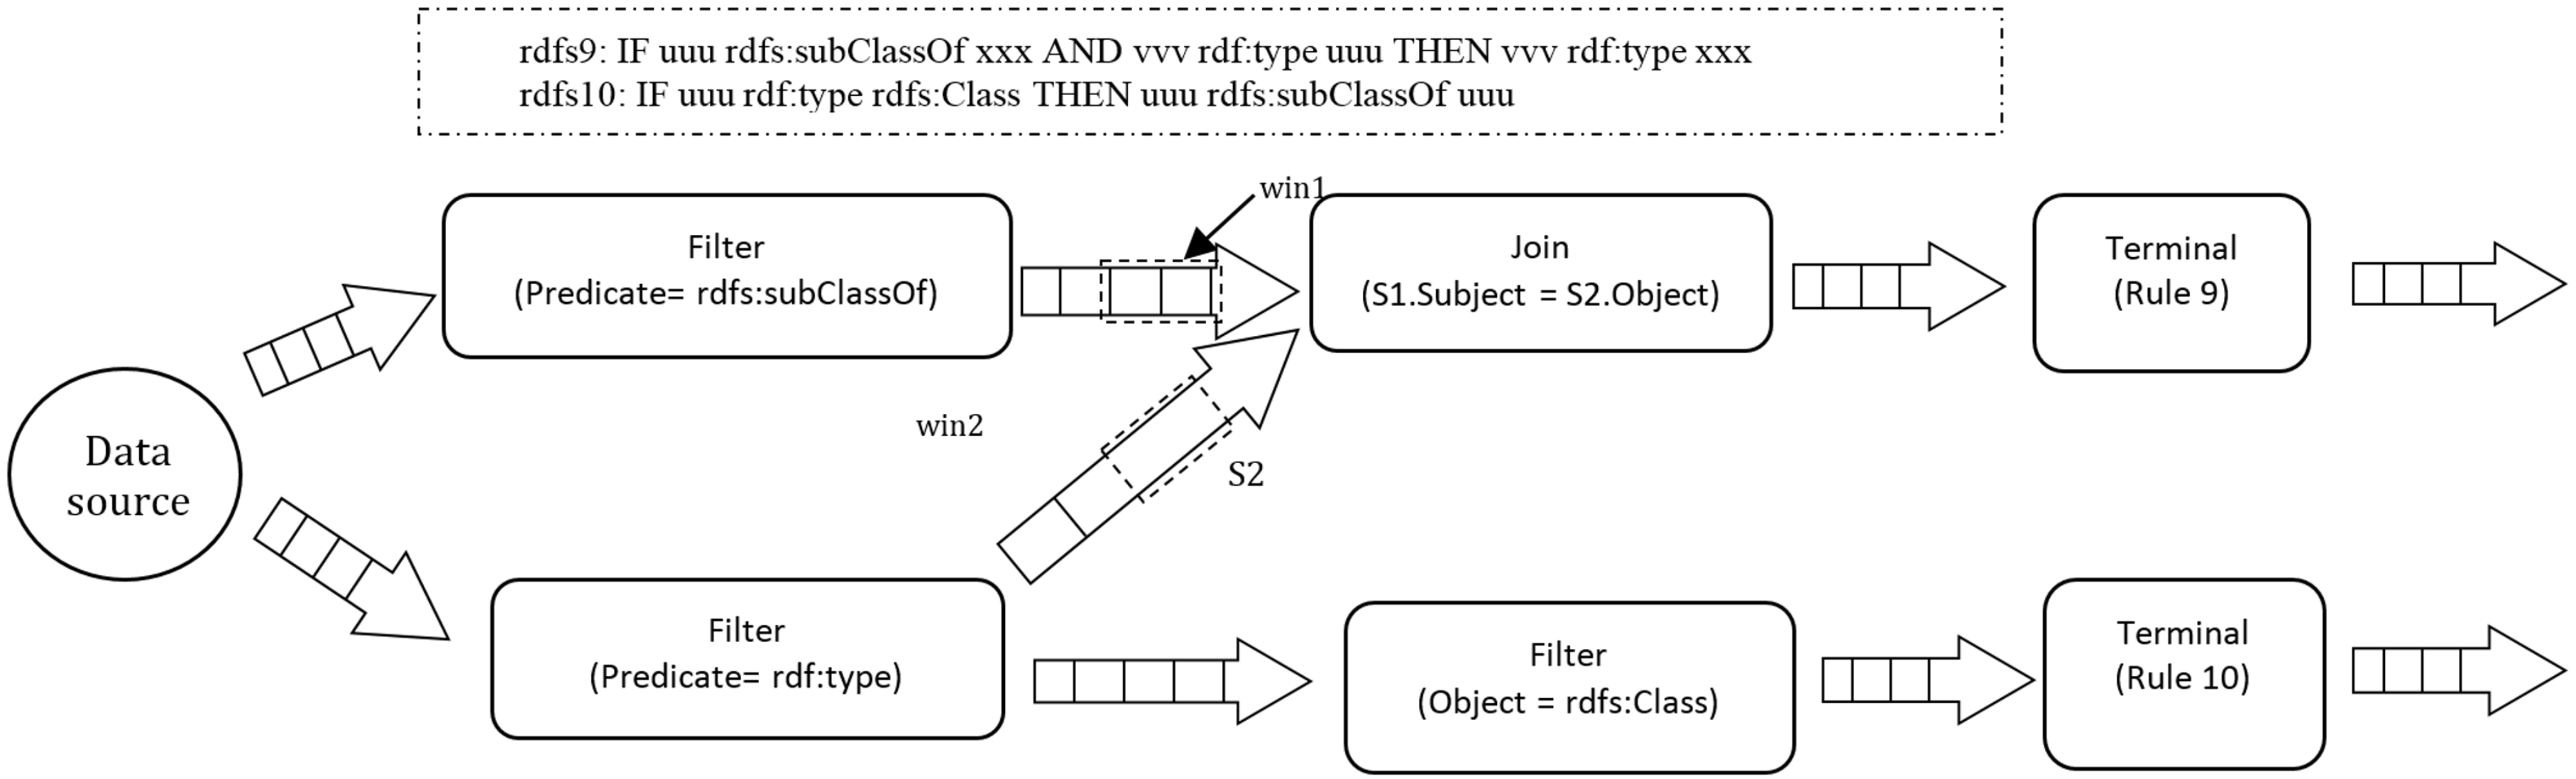
\includegraphics[width=0.9\textwidth]{example-rete-network.png}
      \caption{An example Rete network with corresponding (RDFS) rules.}
      \labelfig{example-rete-network}
    \end{figure*}
    In R4, data enters the network through the source nodes, which convert streams of graphs into streams of quads, by extracting the graph ID and attaching it to every triple in this graph.
    Source nodes are, therefore, implementations of the graph-to-stream operator ${{}_g{\pi_t}}$ of CoDeR.
    Source nodes also annotate the incoming quads with the system time at their arrival if their parent graph was not already annotated at its origin, otherwise passing the annotation of the graph to the resulting quads.
    This annotation $a$ relates to their instant of assertion $e$ within the CoDeR data model, and the instant $n$ at which they will leave the window whose range $r$ is defined in the system's rule set may be derived by ${n = a + r}$.
    Source nodes propagate the annotated quads to their successor nodes, which are the alpha nodes.

    Alpha nodes are single-entry nodes that form a discrimination network, as shown in \reffig{example-rete-network}.
    In R4, alpha nodes can receive streamed quads from any number of nodes through its single input, reflecting the multiple-source nature of CoDeR's streams.
    Each received quad is matched against some conditions, and is either dropped if there is no match, or propagated downstream to its successor node(s) in the case of a match.
    As such, R4's interpretation of alpha nodes are implementations of the triple-select operator $\sigma_{triple}$ of CoDeR, but can also filter based on the datatypes of the values in triples, thereby also implementing the other selection operator of CoDeR, $\sigma_{external}$.

    The first alpha node in the network propagates matched quads to a special node called the left input adaptor, while the other alpha nodes propagate their output directly to beta nodes.
    The left input adaptor node is responsible of preparing the incoming quads to enter the beta network from the left input of the first beta node in a given join-tree.
    It creates a new \emph{token} that represents a partial match, defined as a list of quads, for each rule body for which the incoming quad is a sub-graph match, then adds this quad as the first item in each list.
    It also annotates each token with the same time as was the quad for which it was generated.
    Tokens are then sent to the first nodes in the beta network.

    Beta nodes are two-input nodes that are responsible for joining the branches of the alpha network, as demonstrated in \reffig{example-rete-network}.
    In our implementation, as in the original Rete algorithm, beta nodes form a left-deep tree.
    Each beta node maintains a left memory, which is a beta memory storing tokens received from other beta nodes (or from the left input adaptor node in case of the first beta node) and a right memory, which is an alpha memory storing quads received from alpha nodes.
    Join nodes are beta nodes that match graphs from both sides according to some conditions, e.g. a shared variable binding.
    As explained earlier, we use stream-to-stream window-join operators to avoid storing and operating over all partial results.
    In this context, each left (beta) and right (alpha) memory is implemented as a \emph{valid window}.
    These windows are implemented as priorities queues in which quads are ordered according to their time annotations, and pruned by ``popping'' from the queue and deleting any quads whose annotation $a \leqslant i - r$, where $i$ is the current system time and $r$ is the range of the semantic window.

    When a join node is left-activated, i.e. it receives a token through its left input, it first adds the new token to its left window, then it prunes its right window before iterating over the remaining quads to find any matches.
    When a match is found, a new token is created by duplicating the left token and adding the right quad to the new token's quad list.
    The new token is annotated with the \emph{earliest} time with which its component quads were annotated, and then propagated to the next beta node, or to the terminal node if it is in the root node of a join tree.
    Conversely, when the join node is right-activated by receiving a quad from an alpha node, it adds the new quad to the right window, prunes the left window then matches the quad against the remaining tokens.

    This method of annotating tokens with the earliest assertion time of those of its components initially appears to violate the annotation semantics for entailed fact instances laid out in \refsec{semantics,model}.
    However, the ordering of tokens in their streams and the system time $i$ at which they are propagated through the system expresses implicitly CoDeR's entailment time $e$ of entailed instances.
    This leaves the annotation $a$ of a token in R4, in combination with the range $r$ of the semantic window associated with the rule set, able to express CoDeR's negation time ${n}$ of entailed instances by the same calculation as those of asserted instances: ${n = a + r}$.
    As such, the interpretation of beta nodes in R4 is a valid implementation of the window-join operator characterised as a pair of CoDeR SteMs $\rstreamjoin$ implicitly unioned by contribution to the same stream, as shown in \reffig{CoDeR: SteM}.

    Finally, terminal nodes receive tokens from the root nodes of join-trees and are responsible for producing entailed graphs, directly implementing the instance entailment operator $\text{:-}_{head}$ of CoDeR.
    As with the $\text{:-}_{head}$ operator, the annotation of these entailed graphs is directly inherited from the completed token from which it is produced.
    The union of the output of all terminal nodes is both the output of the system itself, and re-entered as an input stream to the source nodes to support iterative inference.
  \end{nestedsection}
\end{nestedsection}

\begin{nestedsection}{Evaluation, Results and Discussion}{evaluation}
  To evaluate the performance of R4, we compare it with state-of-the-art systems that provide the capability of performing background reasoning to some extent on streamed semantic data.
  These include Etalis \citep{EP-SPARQL}, Sparkwave \citep{sparkwave}, Streaming knowledge bases \citep{walavalkar08streamingkb}, and the incremental reasoner presented in \citep{inc-reasoning-background-knowledge}.
  To the best of our knowledge, the latter two implementations were never made public, so we compare R4 against Etalis and Sparkwave only.
  The experiments are performed on an Intel Core i5 computer with 3.2 GHz and 8 GB memory.
  We set up Jtalis (the Java wrapper of Etalis) over SWI-Prolog v7.2.1 and installed Sparkwave v0.5.1.

  \begin{nestedsection}{Comparative Results}{evaluation: comparative results}
    \begin{figure*}[t]
      \centering
      \begin{verbatim}
Forall ?offer ?product ?vendor ?price ?from ?to ?delivery ?webpage(
    If And( ?offer [rdf:type -> bsbm_voc:Offer]
            ?offer [bsbm_voc:product -> ?product]
            ?offer [bsbm_voc:vendor -> ?vendor]
            ?offer [bsbm_voc:price -> ?price]
            ?offer [bsbm_voc:validFrom -> ?from]
            ?offer [bsbm_voc:validTo -> ?to]
            ?offer [bsbm_voc:deliveryDays -> ?delivery]
            ?offer [bsbm_voc:offerWebpage -> ?webpage]
            ?offer [dc:publisher -> ?publisher]
            ?offer [dcc:date -> ?date] )
    Then ?product [bsbm_voc:offerPrice -> ?price] )
      \end{verbatim}
      \caption{The RIF-Core rule inspired by the Berlin SPARQL benchmark.}
      \labelfig{BSBM-rule}
    \end{figure*}

    In order to compare the efficiency of R4 against both Etalis and Sparkwave, we formulated an experiment using the synthetic dataset from the Berlin SPARQL Benchmark \citep{BSBMresults} which was used in the Sparkwave paper.
    We used another 1.1 million triples dataset using the provided data generator, containing information about 100,000 limited-time offers made available by some fictional online marketplace.
    We used a small schema that has 329 product types arranged in a 4-level hierarchy.

    The rule we chose to express in each system, shown in \reffig{BSBM-rule}, entails the offer price for all products that are on offer.
    As offers may be associated with product super-types, some small degree of background reasoning is needed to determine the offer price for specific product sub-types.

    Before we move on to more detailed analysis of the results, we noticed that this rule takes significantly longer to process in Etalis (3 hours for the 1.1 million dataset with 1 second time window compared to ${<10}$ minutes for the other two systems).
    However, when we changed the `And' into a series of `seq's, the system runs 20x times faster (7.5 minutes for the same test).
    Such a drastic difference is likely to be caused by the optimisation of Etalis for the \emph{seq} operator: being intended for \emph{event processing} rather than continuous querying/reasoning, the order of arrival of triples is often more relevant than their simple coincidence in the system.
    In order to present results that provide a meaningful comparison between the time efficiency of each system with regards to changing window ranges, as in \reffig{all-systems-varying-windows}, we chose to modify the rule when evaluating Etalis to use \emph{seq} instead of \emph{And}.
    It should be noted that we recognise that this modified rule is not semantically equivalent to that by which we evaluate R4 and Sparkwave, which cannot express the \emph{seq} operator, but is sufficient to contrast the effect of window range on the time-efficiency and memory-consumption of the three systems.
    \begin{figure}
      \centering
      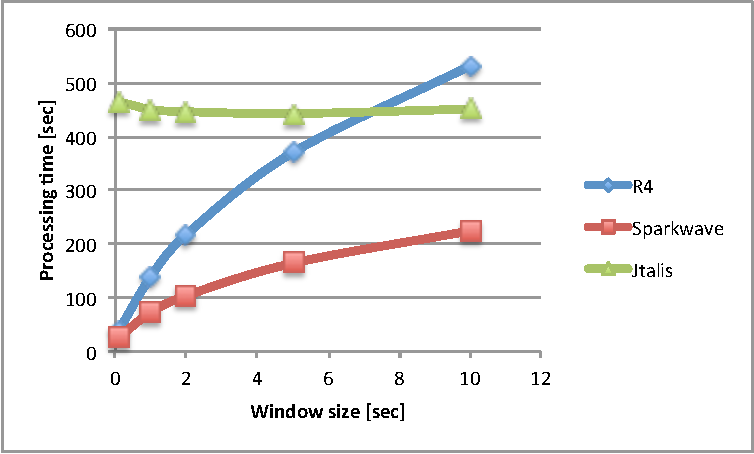
\includegraphics[width=0.45\textwidth]{all-systems-varying-windows}
      \caption{A comparison of the times taken by the systems R4, Sparkwave and Etalis to process 1.1 million triples from a single input stream, given windows of various ranges over the input stream.}
      \labelfig{all-systems-varying-windows}
    \end{figure}

    As shown in \reffig{all-systems-varying-windows}, R4 is faster than Etalis for small windows but slower than Sparkwave, and, while the time-to-complete increases with window range in both Sparkwave and R4, that of Etalis appears to remain fairly constant for the window ranges tested.
    The growing difference between R4 and Sparkwave as the range of the windows increases is likely due to the fact that Sparkwave uses a hash-join algorithm with garbage-collection window-maintenance while the current implementation of R4 uses loop-joins over lists maintained by indexing over time annotations;
    as data remains valid for longer, the beta memories (i.e valid windows) grow bigger, and window-joins in R4 need significantly longer to iteratively check for matches compared to the hash-based look-up of those in Sparkwave.
    More time-efficient, multi-index window-joins are to be considered for R4 in future work.

    We also examined the memory consumption of R4, Sparkwave, and Jtalis throughout a run.
    Setting the sliding window range to five seconds, \reffig{all-systems-memory-consumption} shows the amount of memory used by the three engines during the life time of the BSBM rule.
    It shows that, while R4 and Jtalis follow similar patterns, Sparkwave's memory needs are significantly higher and continue to increase over time, a behaviour that should not occur when applying windows over streams.
    Though we cannot know the reason for this without a thorough inspection of the Sparkwave code-base, we suspect that this is related to an interaction between the manual garbage collection performed by Sparkwave and the underlying JVM garbage collector.
    \begin{figure}
      \centering
      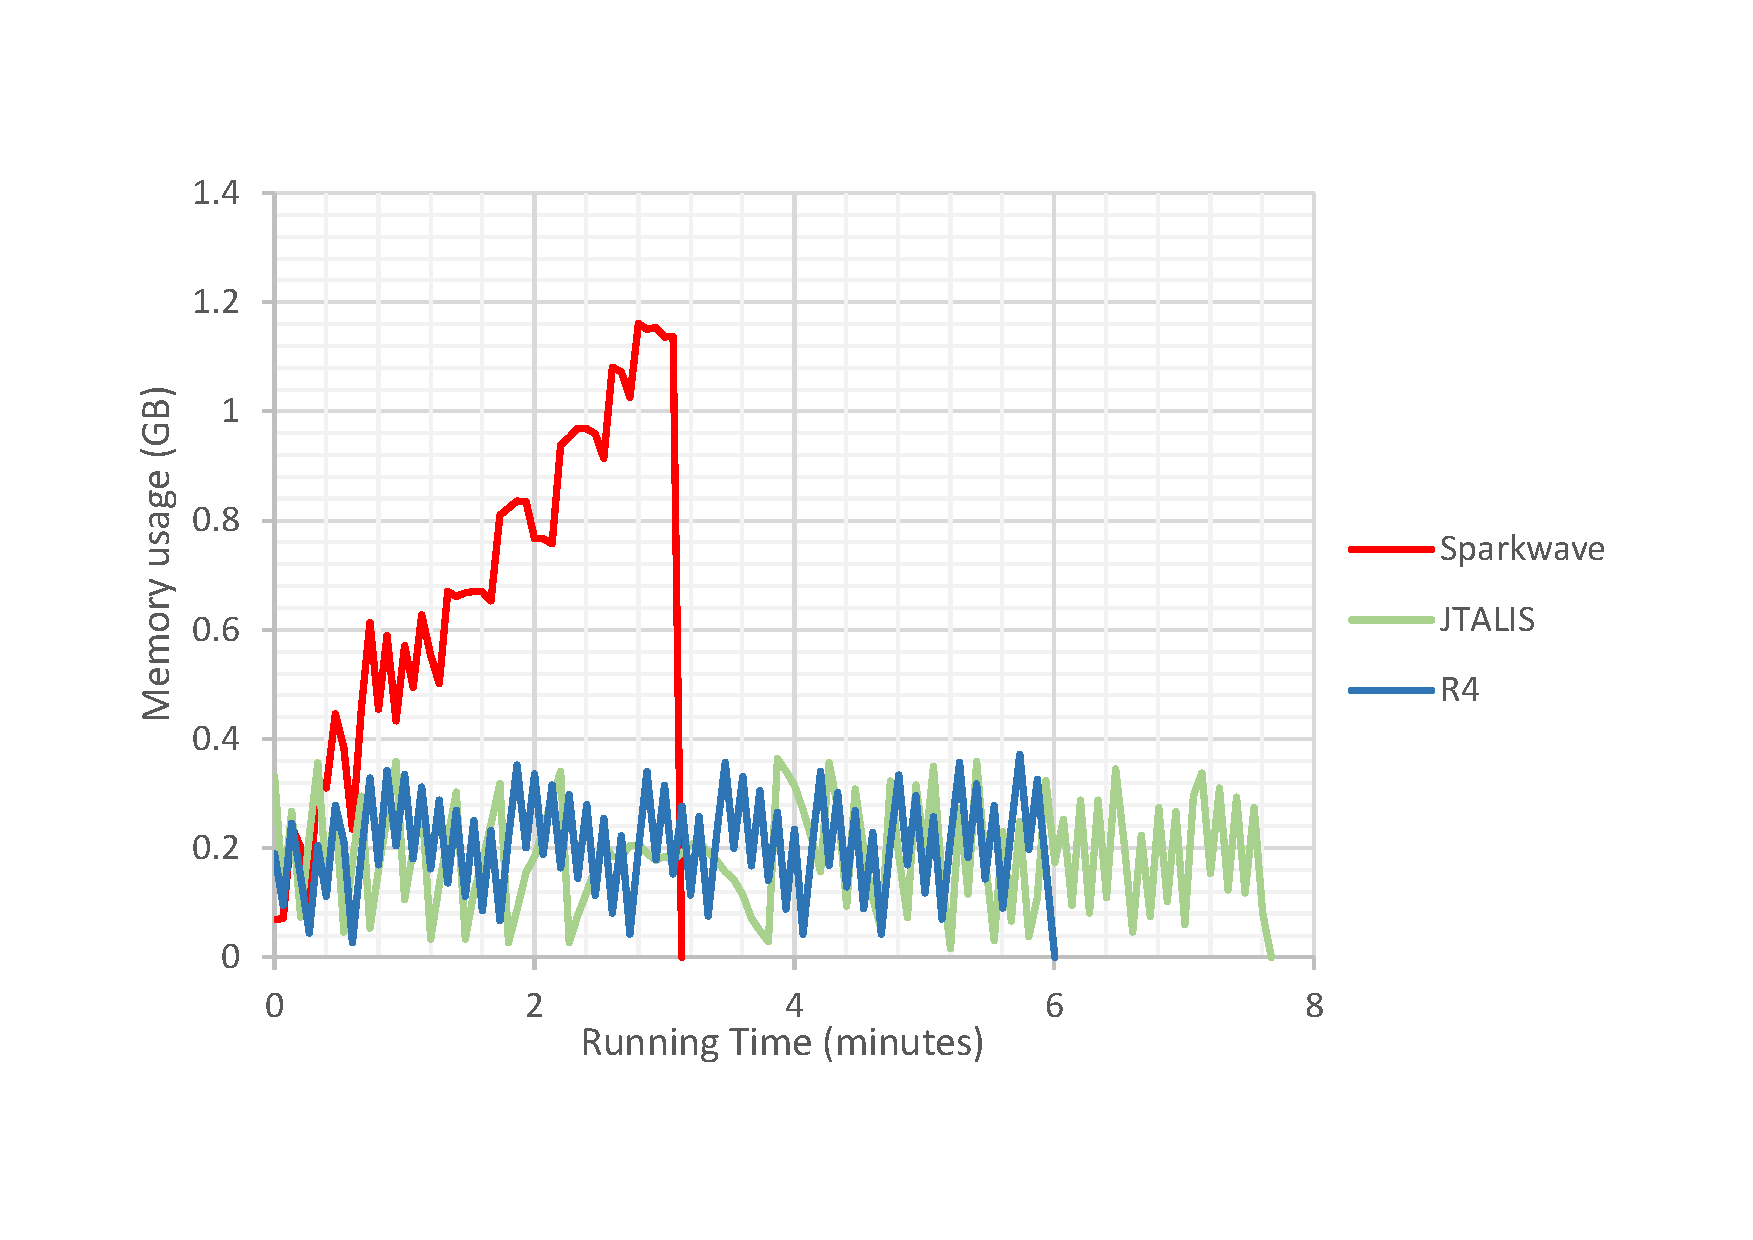
\includegraphics[width=0.5\textwidth]{memoryConsumptionComparison}
      \caption{A comparison of the memory consumed by the systems R4, Sparkwave and Etalis throughout a run processing 1.1 million triples from a single input stream, given sliding windows of 10 seconds over the input stream.}
      \labelfig{all-systems-memory-consumption}
    \end{figure}
  \end{nestedsection}
\end{nestedsection}

\begin{nestedsection}{Conclusions}{conclusions}
  We have presented Windowed Continuous Datalog (\emph{WC-Datalog}), a semantics for stream-based reasoning and streamed entailments at the expressivity of OWL 2 RL, extended incrementally from that of positive Datalog with temporal annotation, streams and windowing semantics.
  In this way it differs from temporal interpretations of Datalog \citep{OrgunWadge92,Tuzhilin93} in that it forgoes the concepts of conventional temporal reasoning, instead applying temporally-agnostic rules to global sliding windows over streams as in stream querying, and casting a continuous program as a series of discrete states.
  WC-Datalog explicitly supports the derivation of sets of facts as the entailment of each discrete state of a continuous program \emph{and} the derivation of concise streams of facts as the entailment of a continuous program over time, in a similar manner to the \emph{RStream}, \emph{IStream} and \emph{DStream} operators of the CQL continuous query language \citep{CQL}.
  In addition to this, however, it also supports the low-complexity derivation of the entailment of each discrete state from the streamed entailment of the continuous program via the application of sliding windows to the concise streams, leading to the definition of a \emph{valid window} over the combined streams $P$ and $N$.
  Thus WC-Datalog represents a semantics not only for low-complexity continuous reasoning, but for \emph{concise} streamed entailments of continuous programs, suitable for consumption in further stream processing without loss of temporal information.

  In order to express this semantics we have developed CoDeR, a processing model for \emph{Co}ntinuous \emph{De}ductive \emph{R}easoning over RDF.
  This processing model is composed of a stream-based data model with a dual semantics and a stream-to-stream extension of a semantic interpretation of the relational algebra.
  The data model is composed of streams of RDF graphs annotated both with the time at which they became valid and the time at which they will cease to be valid, with the ordering of graphs by the former being the sequence of facts in $P$ and the ordering by the latter being the sequence of facts in $N$, hence providing a dual semantics for the stream.
  As such, the windows inherent in a windowed continuous program may be represented in the annotation of each graph in the streamed input, rather than ranged window operators in the algebra.
  Instead, the algebra makes use of \emph{valid window} operators to maintain the set of graphs that are both considered to be true at a given moment \emph{and} applicable at a given point in the processing.
  It also de-constructs the conventional window-join operator of stream-to-stream algebras for continuous querying into the union of the outputs of complementary State Modules (\emph{SteMs}) \citep{SteMs}, to which it is logically and functionally equivalent, thereby supporting greater variety in the possible plans that express a given continuous program.

  Finally, we have implemented the CoDeR model in the synchronous RDF stream-reasoning system R4.
  R4 utilises a variant of the Rete pattern matching algorithm \citep{forgy79} to produce processing plans for sets of rules expressed in RIF-Core \citep{w3crifcore}, the W3C recommendation for expressing sets of rules with the semantics of positive Datalog and the rule language used to express the set of entailment rules of OWL 2 RL \citep{w3cowl2profiles}.
  R4 is sound and complete with respect to the semantics of WC-RIF-Core by virtue of implementing CoDeR.
  Given that there are no benchmarks for more expressive stream-based reasoning, we contrasted the time efficiency and memory consumption of R4 with those of Sparkwave \citep{sparkwave} and Etalis \citep{EP-SPARQL} using a modification of the big-data/RDFS benchmark BSBM \citep{BSBMresults}.
  We have demonstrated that R4 is faster than these RDF stream-querying systems, without loss of comparative soundness or completeness, when applying low-range windows to high-throughput streams, despite Sparkwave and Etalis supporting more limited/less explicitly well-grounded reasoning than that of R4.

  Moving forward, we plan to investigate alternate planing algorithms to improve the Quality of Service (\emph{QoS}) characteristics of the system, i.e. reduce the latency from receipt of some new graph to the production of entailments justified in part by that new graph.
  These primarily focus on the use of SteMs outside of the composition of window-joins, either taking an adaptive approach \citep{eddies,CACQ,CQELS} or utilising the wider array of static plans such an operator affords.
\end{nestedsection}

  \section*{References}
	\bibliographystyle{elsarticle-harv}
	\bibliography{bibliography}
\end{document}
